\documentclass{../../text-style}

\texttitle{Лекция 1: Введение в робототехнику}

\begin{document}

\maketitle
\thispagestyle{empty}

\section{Введение}

Робототехника --- это наука об автономных технических системах, точнее, наука о разработке и применении роботов.
Правда, что такое автономные технические системы или роботы, консенсуса особого нет.
Вообще, слово \enquote{Робот} использовал ещё Карел Чапек в 1920-м году, в своей пьесе \enquote{Россумские универсальные роботы}, ещё когда даже компьютеров не существовало.
Под роботами обычно понимаются \enquote{автоматические устройства, предназначенные для осуществления различного рода действий, обычно выполняемых человеком}%
\footnote{Определение из Википедии, URL: \url{https://ru.wikipedia.org/wiki/Робот} (дата обращения: 08.02.2024).}%
, однако это вызывает больше вопросов, чем ответов. Например:

\begin{itemize}
    \item почтовый робот --- это автономная и, очевидно, техническая система, но всё-таки не то, про что будет речь в этом курсе;
    \item игрушки роботы-собаки не делают действий, обычно выполняемых человеком, но скорее роботы, чем нет;
    \item посудомойка --- автоматическое устройство, которое моет посуду, но не робот.
\end{itemize}

Мы, следуя традициям кибернетиков СПбГУ, будем называть роботами автономные автоматические устройства с замкнутым циклом управления с обратной связью, то есть устройства, способные действовать без участия человека (замкнутость цикла управления) и реагировать на изменения во внешней среде (обратная связь).
Обратите внимание, что, например, робот-сапёр с дистанционным управлением по нашему определению роботом не является, поскольку требует человека в контуре управления.
Однако это тоже не то чтобы точное определение, потому что, например, насосная станция поддерживает давление в водопроводе без участия человека, но не робот (а автомат).
Но думаю, что идея понятна, тем более что в этом курсе речь пойдёт прежде всего про мобильные роботы, в этой сфере понятие робота более определённо.

Кстати, насчёт кибернетиков.
\emph{Кибернетика} в общем смысле --- наука об управлении, изучает законы управления, взаимодействие управляющей и управляемой систем, информационные потоки и т.д. и т.п.
Это раздел прикладной математики, который имеет весьма опосредованное отношение к инженерии и, на самом деле, даже к робототехнике, поскольку кибернетика вполне применяется в таких нематериальных вещах, как экономика.
Кибернетикой мы в этом курсе заниматься не будем (только чуть-чуть коснёмся), но вообще на матмехе СПбГУ есть аж две кафедры кибернетики (теоретической и прикладной), с очень давней и очень славной историей, напрямую связанной с робототехникой (что интересно, робототехникой в основном занимаются как раз теоркибернетики).

\subsection{Какие роботы бывают}

Немного поговорим про типы роботов, используемые в разных областях народного хозяйства. 
Вообще, их можно разделить на два крупных класса --- стационарные роботы (манипуляторы) и мобильные роботы.

Как ни странно, в промышленности в основном используются именно стационарные роботы, то есть идеи писателей-фантастов про железных человекоподобных рабов, которые в конечном итоге восстают и уничтожают человечество, не нашли пока практического применения.
Реальный промышленный робот --- это манипулятор, намертво привинченный к полу, например, популярная серия роботов-манипуляторов KUKA:

\begin{center}
    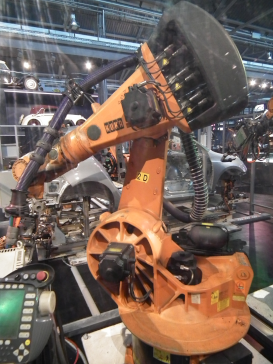
\includegraphics[width=0.4\textwidth]{kuka.png}
\end{center}

Несмотря на невпечатляющий внешний вид, это вполне робот, то есть автономная система, имеющая датчики и способная реагировать на изменения в окружающей среде.
В промышленных применениях основное изменение окружающей среды, на которое надо реагировать --- это появление препятствия в рабочей зоне (например, человека, которого желательно не зашибить, хотя для этого рабочую зону обычно просто огораживают).
Такие роботы используются в самых разных технических процессах, начиная от нанесения покрытия на деталь (когда её надо в течение пары десятков часов с равномерной скоростью вытягивать из раствора, на что человек в принципе не способен) заканчивая привинчиванием колёс к автомобилю.

Вот несколько более странно выглядящий робот-манипулятор:

\begin{center}
    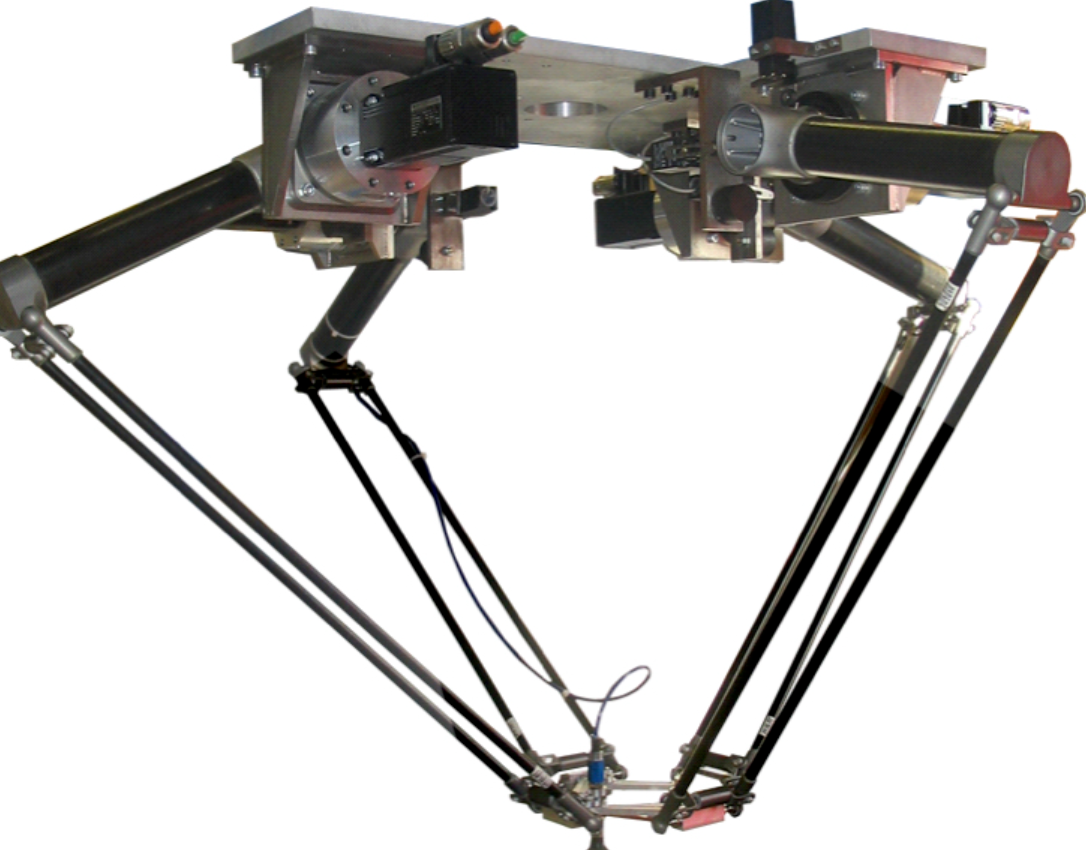
\includegraphics[width=0.4\textwidth]{delta.png}
\end{center}

Это один из так называемых дельта-роботов, которые хороши тем, что могут точно позиционироваться в трёхмерном пространстве, поэтому используются в точных производствах, например, монтаже печатных плат.
На них также есть датчики, которые часто используются для точного измерения пространственного положения манипулятора и его корректировки.

В этом курсе больше внимания будет уделено мобильным роботам.
Они тоже делятся на целый ряд сильно непохожих друг на друга типов:

\begin{itemize}
    \item Колёсные или гусеничные --- от робота-пылесоса до марсохода, широко используются и в промышленности (складские роботы), и в быту, стандарт де-факто в научных работах по робототехнике в силу простоты, практичности и эффективности.
    Беспилотные автомобили тоже попадают в эту категорию.
    \item БПЛА --- новый тренд в робототехнике, используемый в военном деле, сельском хозяйстве, для обнаружения лесных пожаров, контроля состояния трубопроводов, построения карт и трёхмерных моделей местности и т.д. и т.п.
    В основном сейчас распространены дистанционно управляемые беспилотные аппараты, которые, несмотря на развитую автоматику для поддержания положения в пространстве, роботами в смысле этого курса назвать нельзя.
    Однако среди БПЛА встречаются и роботы в самом полном смысле этого слова, БПЛА также любимы учёными-робототехниками за \sout{возможность записывать впечатляющие видео по групповому взаимодействию беспилотников} отличную мобильность и огромную потенциальную полезность в хозяйстве.
    БПЛА в свою очередь делятся на:
    \begin{itemize}
        \item аппараты условно вертолётного типа --- квадрокоптеры, гексокоптеры и т.п.; тогда как настоящие вертолёты (то есть аппараты с автоматом перекоса) используются крайне редко в силу сложности и дороговизны требуемой механики;
        \item аппараты с фиксированным крылом (к ним же в целом можно отнести конвертопланы).
    \end{itemize}
    Квадрокоптеры дёшевы, просты и очень мобильны, но ограничены в автономии, аппараты с фиксированным крылом могут хоть бесконечно находиться в воздухе (см., например, Airbus Zephyr).
    Кстати, современные (и не очень) крылатые ракеты вполне можно считать роботами --- навигация по рельефу местности в них была реализована ещё в 70-х годах 20-го века (см. BGM-109 \foreignquote{english}{Tomahawk}).
    \item Надводные и подводные роботы --- по задачам и особенностям управления весьма схожи с БПЛА, но имеют гораздо более узкую сферу применения.
    \item Шагающие роботы --- эффектны (см. роботы Boston Dynamics), способны работать на пересечённой местности, но очень сложны в управлении и довольно неэффективны.
    На практике особо не применяются, хотя R. Siegwart в своей книге приводит вот такую штуку для лесозаготовок:
    \begin{center}
        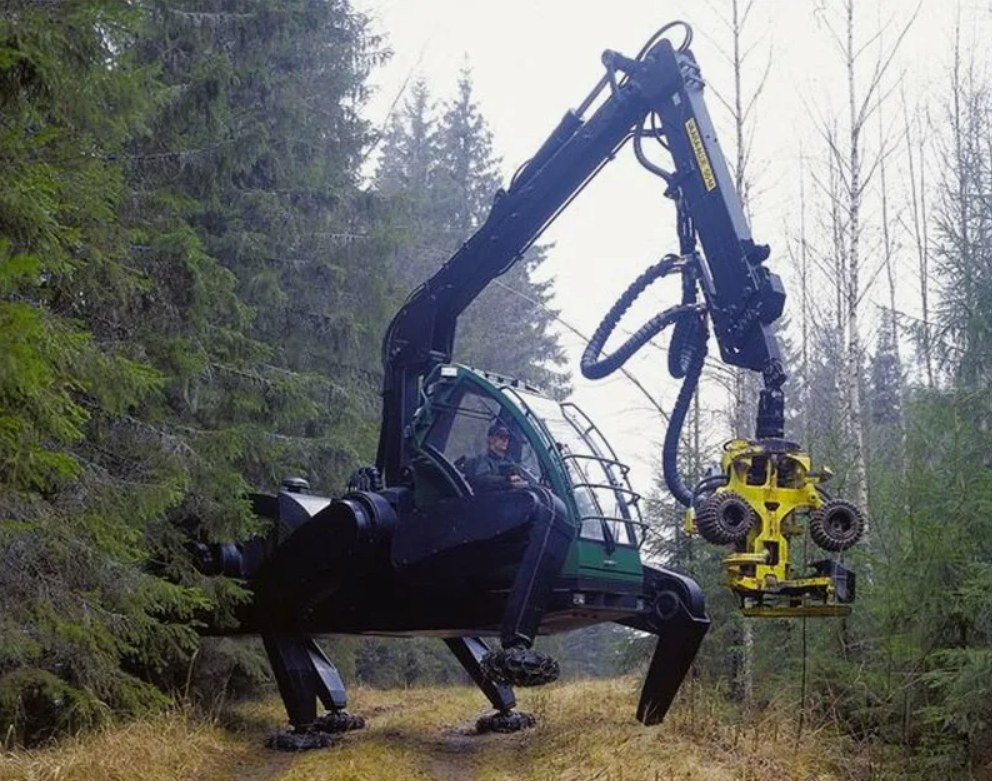
\includegraphics[width=0.5\textwidth]{plustechWalker.png}
    \end{center}
    Это не робот в нашем понимании, поскольку требует оператора (хотя сам управляет ногами), но шагающий и якобы полезный, поскольку может двигаться в непролазных чащобах, где у колёсной и даже гусеничной техники нет шансов.
\end{itemize}

\subsection{Робототехника на матмехе}

На матмехе робототехникой занимаются давно и довольно успешно, также вокруг матмеха есть довольно много сильных команд в этой области, занимающихся исследованиями вполне мирового уровня.
Для чего, собственно, и проводится этот курс --- дать обзор, ввести в курс дела, заинтересовать, чтобы в магистратуре можно было к этим исследованиям присоединиться.
Чем занимались (и занимаются) на матмехе в плане робототехники:

\begin{itemize}
    \item Образовательный конструктор ТРИК для обучения робототехнике и основам программирования школьников и студентов.
    Разрабатывался скорее \enquote{вокруг} матмеха, отдельной компанией, где не все были матмеховцами, но начиналось всё из коллаборации преподавателей кафедры теоретической кибернетики и системного программирования, и они же всегда были главной движущей силой проекта.
    Конструктор ТРИК широко известен в школьной робототехнике, признан как официальный для ряда олимпиад, используется в школьном образовании и в зарубежье.
    Вот пример робота-тележки ТРИК:
        \begin{center}
            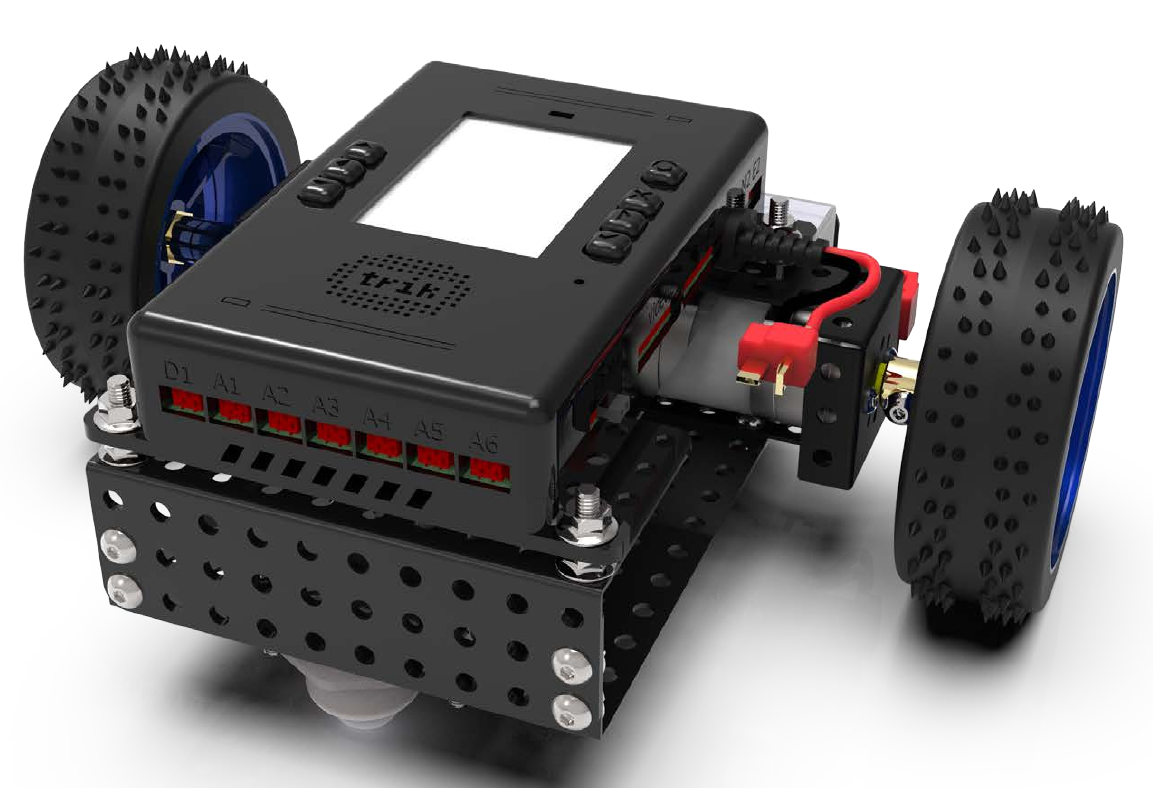
\includegraphics[width=0.5\textwidth]{trik.png}
        \end{center}
    \item Среда программирования TRIK Studio/QReal:Robots --- визуальная система программирования для образовательной робототехники, изначально создавалась для конструктора Lego Mindstorms NXT, потом там появилась поддержка Lego Mindstorms EV3 и ТРИК, потом и ряда других конструкторов.
    Тоже пошла в народ, тоже признана как официальная среда программирования на олимпиадах, на её основе записано вроде как несколько онлайн-курсов (для Stepik), защищена одна диссертация.
    \item Ресурсный центр \enquote{Робототехника и БАС} --- недавно созданный ресурсный центр СПбГУ, тоже не совсем на матмехе, там занимаются в основном беспилотниками.
    \item Кафедра теоретической кибернетики профессионально занималась робототехникой ещё до того, как все мы родились, причём занималась не только фундаментальной наукой, но и строила свои роботы.
\end{itemize}

\section{Алгоритмические основы}

Этот курс в называется \enquote{Алгоритмические основы робототехники}, поэтому с алгоритмических основ и начнём.
Алгоритмы в роботах нужны для управления, в самом широком смысле, от управления моторами до планирования миссии.
Управление в целом работает по стандартной схеме, описываемой архитектурным шаблоном \enquote{Sense-Compute-Control}:

\begin{center}
    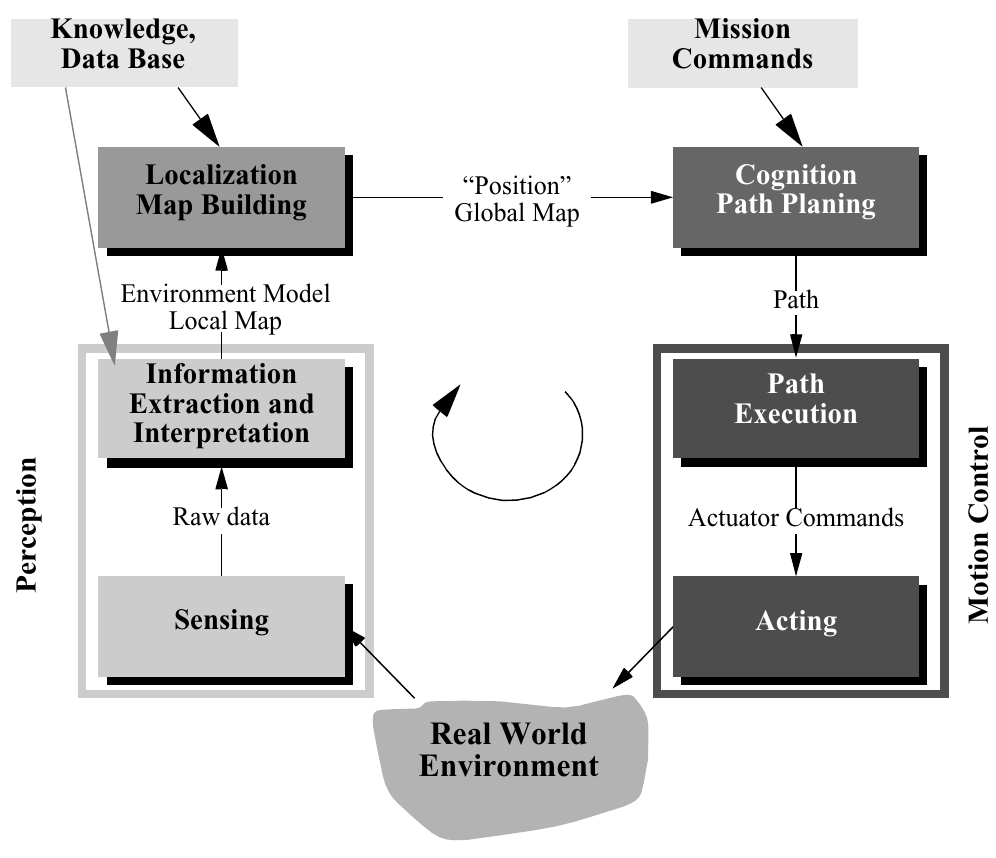
\includegraphics[width=0.7\textwidth]{controlLoop.png}
    \attribution{R. Siegwart, I.R. Nourbakhsh, Introduction to Autonomous Mobile Robots}
\end{center}

Реальный мир воспринимается сенсорами, из их показаний извлекается и интерпретируется информация.
Это на самом деле важный и нетривиальный этап работы бортового программного обеспечения --- коллеги с кафедры теоретической кибернетики приводили аналогию, что робот похож на человека, сидящего в бочке, и вынужденного по числам, показываемым приборами, строить картину мира вокруг.
Дальше, если это требуется, выполняется локализация или какой-то другой метод понять, в каком состоянии мы сейчас находимся.
Дальше, принимая во внимание поставленную задачу, мы должны понять, что именно надо делать дальше --- например, проложить маршрут к целевой точке.
По проложенному маршруту мы должны рассчитать управляющие воздействия на \emph{актуаторы} --- устройства, которые могут воздействовать на окружающий мир, например, двигатели моторов.
Ну и, наконец, обеспечить подачу рассчитанных управляющих воздействий до следующей итерации цикла управления.
При этом робот взаимодействует с реальным миром (например, перемещается в нём), действия робота приводят к ответной реакции реального мира, которая в свою очередь воспринимается сенсорами робота (результат перемещения --- изменение показаний камер или дальномеров, например).

Принципиальное отличие от программного обеспечения тут в том, что цикл управления вынужден взаимодействовать с реальным миром, который вообще плохо поддаётся оцифровке и алгоритмизации.
Сенсоры неизбежно шумят и врут.
Актуаторы неизбежно отрабатывают не точно.
При локализации неизбежны ошибки, причём они могут быть весьма значительными и приводить к весьма неприятным последствиям%
\footnote{См., например, известный инцидент, когда из-за навигационной ошибки в 1991 году американские вертолёты открыли огонь по своим: \url{https://www.govinfo.gov/content/pkg/GAOREPORTS-OSI-93-4/html/GAOREPORTS-OSI-93-4.htm} (дата обращения: 09.02.2024). Это были не роботы, но навигация для роботов ещё сложнее.}.
И реальный мир имеет свойство изменяться как в ответ на действия робота, так и сам по себе --- например, в окружении робота может быть много подвижных объектов, которые по показаниям сенсоров очень сложно отличить от стационарных, так что построение карты оказывается очень нетривиальной задачей.

Поэтому для роботов необходимы сложные алгоритмы управления.
Но начнём мы с простых.

\subsection{Регуляторы}

В самых простых ситуациях управление сводится к формальной математической задаче: имея установочное значение (то есть, например, желаемое показание датчика), вырабатывать управляющее воздействие (то есть, например, мощность, которую нужно подавать на моторы) так, чтобы система оставалась к установочному значению как можно ближе.
Пример такой задачи --- езда вдоль стены робота, когда мы фиксируем расстояние до стены, которое робот должен поддерживать, и он едет вдоль, не сильно от установленного расстояния отклоняясь.
Или круиз-контроль в автомобиле --- задаём желаемую скорость, автомат поддерживает обороты двигателя так, чтобы автомобиль с этой скоростью двигался, не важно, по прямой или в гору.
Или авиационный автопилот, поддерживающий заданный курс самолёта/БПЛА.

Это классическая задача теории управления, имеющая классические решения --- регуляторы. 
Центробежный регулятор, известный как регулятор Уатта, применялся задолго до Уатта, для управления скоростью вращения двигателей, c 17-го (!) века:

\begin{center}
    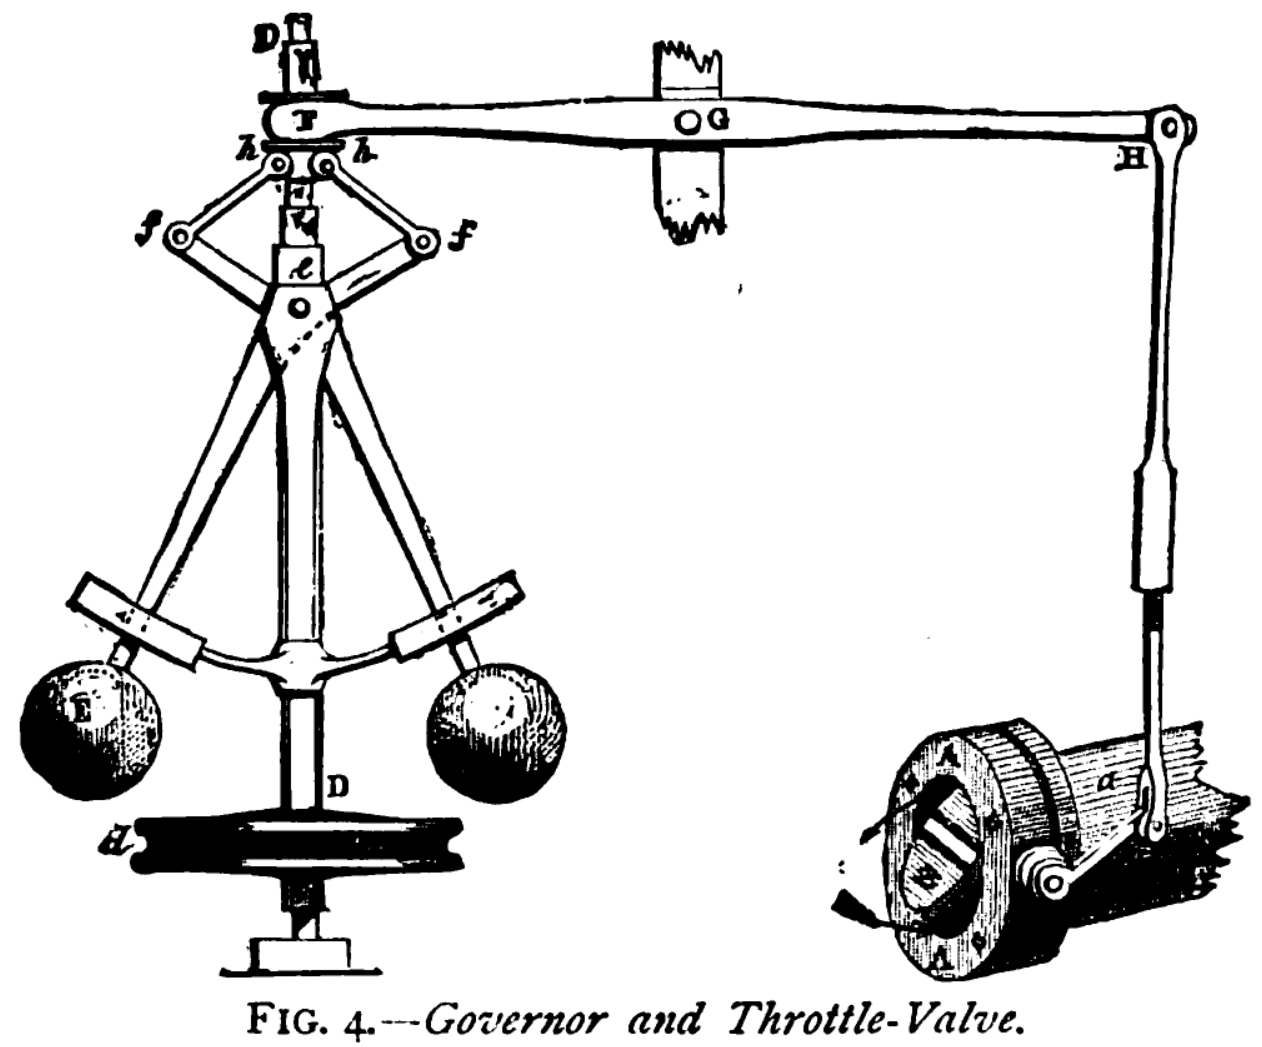
\includegraphics[width=0.6\textwidth]{wattRegulator.png}
    \attribution{\url{https://ru.wikipedia.org/wiki/Центробежный_регулятор}}
\end{center}

Регуляторы бывают разные:

\begin{itemize}
    \item Релейный регулятор работает очень просто --- если значение больше установочного, пытаемся его уменьшить на фиксированную величину, если меньше, пытаемся увеличить.
        Реализуется как обычный if-then, работает плохо, поскольку реальное значение может бесконечно \enquote{прыгать} около установочного, вообще к нему не приближаясь.
    \item Пропорциональный регулятор: управляющее воздействие пропорционально текущему отклонению от установочного значения.
        То есть, например, чем ближе робот к стене, тем активнее он пытается от неё отъехать, чем дальше --- тем активнее подруливает к стене.
        Это позволяет гораздо более точно управлять системой вблизи установочного значения, но при значительных отклонениях система может сильно \enquote{промахиваться}, и кибернетики даже умеют доказывать теорему, что этот процесс не обязательно сойдётся.
    \item Пропорционально-дифференциальный регулятор: управляющее воздействие пропорционально отклонению от установочного значения и скорости его изменения --- например, если робот слишком быстро отворачивает от стены из-за влияния пропорциональной части, дифференциальная часть заставляет его двигаться плавнее, уменьшая \enquote{перепрыгивание} значения.
    \item ПИД-регулятор: управляющее воздействие пропорционально всему выше и длительности пребывания в ошибочном состоянии --- интегральная часть учитывает историю.
        ПИД-регулятор доказанно сходится, всё ещё довольно прост (имеет всего три коэффициента --- перед пропорциональной, дифференциальной и интегральной частью), поэтому используется повсеместно в реальных задачах, в том числе в качестве элементарного строительного блока для более сложных систем управления.
        Например, делать так, чтобы квадрокоптер висел в воздухе винтами вверх, а не хаотично мотался по сторонам, может ПИД-регулятор, а за целенаправленное движение может отвечать более высокоуровневый автопилот, немного \enquote{возмущающий} ПИД-регулятор в правильном направлении.
\end{itemize}

Поскольку мы не углубляемся в теорию управления, изложение намеренно очень неформально --- если интересно, материалов по регуляторам полно, их изучают на кружках по робототехнике в средней школе.

\subsection{Высокоуровневые системы управления}

Если задача требует чего-то более интеллектуального, регуляторами не обойтись, и могут применяться сколь угодно сложные решения. 
\enquote{Продвинутые} решения условно делятся на два класса, основанные на поведении и основанные на локализации.

Основанные на поведении (Behavior-driven)-решения предполагают, что робот не пытается строить детальной модели мира, а непосредственно реагирует на стимулы (все регуляторы, в общем-то, относятся к этому классу).
Несмотря на кажущуюся простоту, behavior-driven-подход широко распространён и вполне подходит для целого ряда содержательных задач.
Например, боты в компьютерных играх (которые не роботы в смысле этого курса, но сойдут за роботов в симуляторе, плюс-минус симуляция шума сенсоров) часто реализуются именно с behavior-driven-системой управления.

\begin{itemize}
    \item Условие-реакция --- поведение робота определяется набором правил из пары \enquote{условие --- действие, которое надо выполнить, если условие истинно}.
    \item Конечные автоматы --- это то же \enquote{условие-реакция}, но с учётом внутреннего состояния робота и возможностью это состояние менять.
        Конечно-автоматная модель немного сложнее, зато гораздо более гибка, чем \enquote{условие-реакция}, поэтому весьма популярна.
    \item Дерево поведений или дерево задач --- иерархическая структура данных, где во внутренних узлах находятся задачи робота (иерархически уточняющие друг друга), в листьях --- конкретные поведения.
        Активно используется в компьютерных играх, поддержаны в популярных игровых движках, хотя создавались (и, конечно, применяются) в робототехнике.
        По сути дерево поведений можно рассматривать как иерархический конечный автомат, только робот не переходит между состояниями, а выбирает задачи.
        Дерево поведений сложнее всех выше рассмотренных подходов в реализации, но гибче всех, плюс позволяет структурировать код в изолированные строительные блоки и комбинировать из них поведение, зачастую с помощью простой визуальной нотации.
\end{itemize}

Основанные на локализации и планировании --- когда робот строит (или заранее имеет) карту (в более общем случае --- вообще некоторую модель) окружающего мира, пытается определить своё местоположение в этой модели и заранее спланировать свои действия так, чтобы оказаться в желаемом положении.
Тут концептуально есть два подхода:

\begin{itemize}
    \item У нас уже есть карта и набор внешних ориентиров, которые позволяют нам найти на карте себя.
    \item SLAM (Simultaneous Localization And Mapping) --- когда карты изначально нет, мы по данным с сенсоров её строим и одновременно с этим локализуемся.
\end{itemize}

В любом случае у нас должно быть некоторое внутреннее представление карты (что само по себе нетривиальная задача, поскольку окружающий мир непрерывен, а любое представление дискретно) и оценка своей позиции на этой карте (именно оценка, потому что сенсоры врут).
По этим данным можно планировать свои действия, например, прокладывать маршрут по карте обычными графовыми алгоритмами (например, \mintinline{text}{A*}).
В этом деле, естественно, есть масса нюансов, начиная от выбора адекватного задаче представления карты и вероятностного представления верований робота о своём местоположении (оно так и называется в англоязычной литературе, \foreignquote{english}{belief representation}) до ограничений, накладываемых кинематической моделью робота.
Собственно, про нюансы (собственно, и составляющие науку \enquote{робототехника}) мы и поговорим дальше.

\section{Кинематика робота}

Кинематика --- это наука о движении безотносительно того, что это движение вызывает. Применительно к робототехнике кинематика нужна, чтобы уметь отвечать на два вопроса:

\begin{itemize}
    \item Прямая кинематическая задача --- есть кинематическая модель робота и набор управляющих воздействий (на низком уровне, типа \enquote{провернуть колесо на столько-то градусов}), какое положение робот займёт в пространстве?
    \item Обратная кинематическая задача --- есть кинематическая модель робота и целевое положение робота, каков набор управляющих воздействий, необходимых, чтобы целевого положения достигнуть?
\end{itemize}

Под кинематической моделью тут понимается устройство \enquote{движущей части} робота --- его колёсная формула, ведущие/не ведущие, управляемые/не управляемые колёса, число сочленений в манипуляторе или ноге, число и расположение винтов и т.п.
Только для наземных роботов, несколько примеров моделей:

\begin{itemize}
    \item Шагающие --- две ноги, как у людей; четыре ноги, как у животных; 6 ног, как у насекомых.
    \item Колёсные --- четыре известных вида колеса, включая \enquote{шведские} и просто шар в лунке, более десятка широкоизвестных конфигураций этих самых колёс: \enquote{автомобильное} управление, когда два колеса связаны трапециевидным механизмом и синхронно отклоняются в стороны (называется рулевой трапецией Аккермана), \enquote{мотоциклетное}, когда есть только одно отклоняемое колесо, дифференциальное (\enquote{танковое}), когда руление выполняется за счёт разности оборотов колёс по разные стороны тележки (обороты вполне могут быть отрицательными, что даёт возможность при такой схеме разворачиваться на месте, в отличие от предыдущих рассмотренных конфигураций), омниколёса (они же шведские колёса, кто ни разу не слышал --- обязательно погуглите), синхропривод.
\end{itemize}

Вот пример кинематической модели, самой хитрой из вышеперечисленных, трёхколёсной синхроприводной тележки:

\begin{center}
    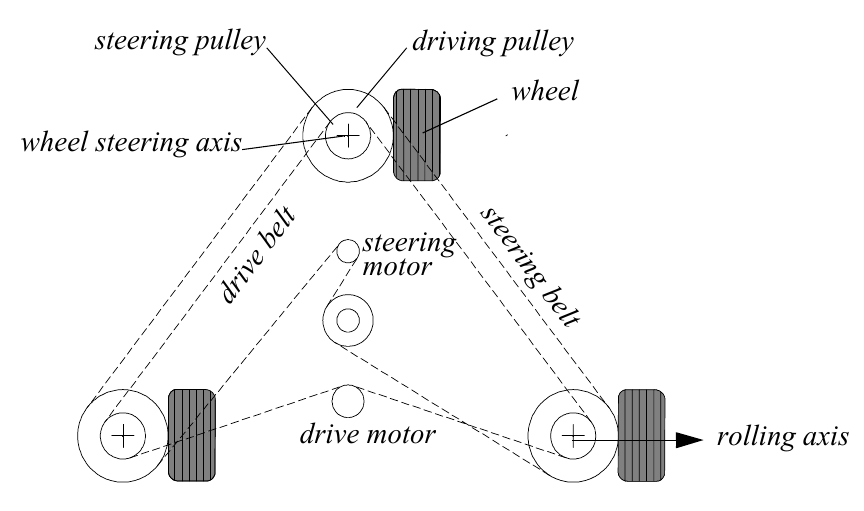
\includegraphics[width=0.7\textwidth]{synchroDrive.png}
    \attribution{R. Siegwart, I.R. Nourbakhsh, Introduction to Autonomous Mobile Robots}
\end{center}

Три колеса управляются двумя моторами, один отвечает за тягу, другой за руление.
Моторы и колёса связаны ременной (или цепной) передачей, что позволяет одному мотору двигать сразу все три колеса.
Схема позволяет поворачивать на месте и довольно точно позиционировать робот, плюс экономить дорогие моторы, но механически сложна, поэтому редко используется.

Например, бытовые роботы-пылесосы в подавляющем большинстве случаев представляют собой трёхколёсные тележки с дифференциальным управлением с двумя ведущими колёсами и одним пассивным (не связанным с мотором) поворотным колесом.

У каждой кинематической модели есть степени свободы --- сколько независимых параметров описывают состояние модели.
Не всегда всеми ими можно управлять.
Например, робот на омниколёсах может независимо менять свои координаты по любой из осей и своё положение в пространстве, у него три степени свободы и все три управляемы.
Робот с автомобильным управлением (например, беспилотный автомобиль) может двигаться вперёд-назад и отклонять рулевые колёса (так что мы управляем двумя переменными из трёх).
Для роботов-манипуляторов степени свободы --- это количество сочленений и степени свободы шарниров, для шагающих роботов --- тоже, но даже если мы можем всеми сочленениями управлять независимо, есть естественное ограничение, что робот не должен упасть, так что фактически управляемых степеней свободы у него принципиально меньше, чем степеней свободы вообще.

Роботы, у которых мы можем управлять всеми их степенями свободы, называются \emph{голономными}, если нет --- соответственно \emph{неголономными}.
Понятие голономности в математике более общо и определяется интегрируемостью уравнений, но в робототехнической кинематике это на самом деле оказывается эквивалентным простому определению выше.

Формально для обсуждения кинематики вводится понятие \emph{позы робота}, то есть расположения его в пространстве.
Например, для трёхколёсной тележки поза описывается координатами в двумерном пространстве и углом поворота робота:

\begin{center}
    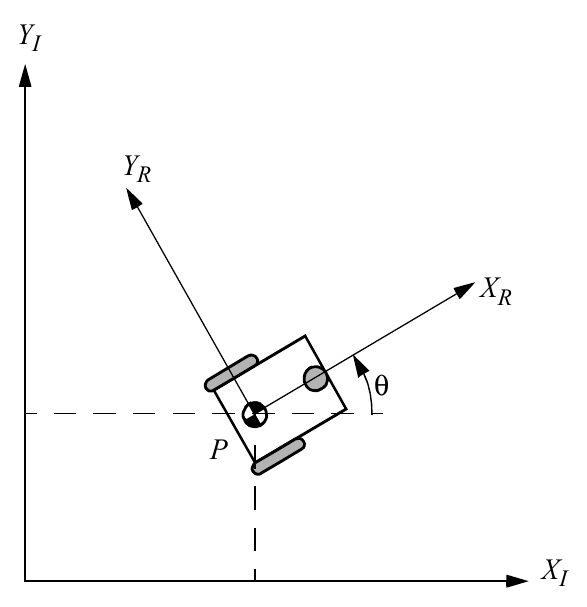
\includegraphics[width=0.5\textwidth]{pose.png}
    \attribution{R. Siegwart, I.R. Nourbakhsh, Introduction to Autonomous Mobile Robots}
\end{center}

Для летающих роботов всё несколько сложнее, для манипуляторов даже ещё интереснее.

Поза всегда оценивается относительно некоторой глобальной системы координат, для трёхколёсных тележек формально в виде вектора
$$\xi_I = \begin{bmatrix} x \\ y \\ \theta \end{bmatrix}$$

Тогда прямая кинематическая модель трёхколёсной тележки формально может быть формально описана как функция от текущей позы робота и управляющих воздействий:

$$\dot{\xi_I} = \begin{bmatrix} \dot{x} \\ \dot{y} \\ \dot{\theta} \end{bmatrix} = f(l, r, \theta, \dot{\phi_1}, \dot{\phi_2})$$

Где $l$ --- дистанция от центра робота до центров колёс, $r$ --- радиус колеса, $\theta$ --- направление робота в глобальной системе координат, $\dot{\phi_1}$, $\dot{\phi_2}$ --- угловые скорости колёс 1 и 2. По такому уравнению можно посчитать перемещение робота в локальной системе координат, а затем транслировать его в глобальную систему координат с помощью матрицы аффинного преобразования, состоящей из двух компонентов --- поворота и переноса.

Однако задача управления несколько сложнее: по текущей и желаемой позе робота построить управление (то есть определить функции $\phi_1(t)$ и $\phi_2(t)$), которые переведут робот из текущей позы в желаемую:

\begin{center}
    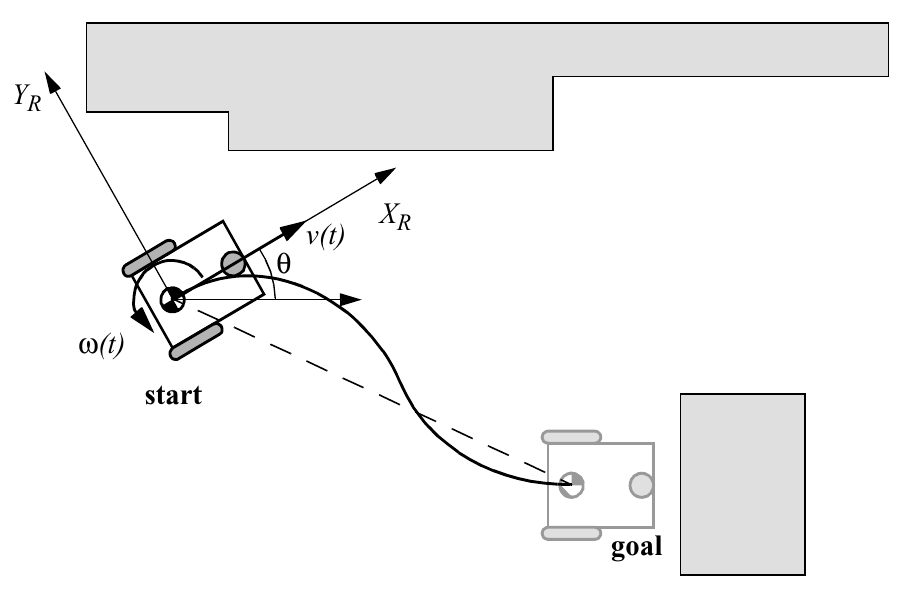
\includegraphics[width=0.8\textwidth]{inverseKinematics.png}
    \attribution{R. Siegwart, I.R. Nourbakhsh, Introduction to Autonomous Mobile Robots}
\end{center}

То есть уравнение прямой кинематической модели приходится решать в обратную сторону, и тут в общем случае не обойтись без суровых дифуров. И напомнит, что речь тут идёт про трёхколёсную тележку с двумя активными колёсами и одним пассивным поворотным, то есть самый простой случай.

\section{Сенсорика}

Теперь, когда мы обсудили то, чем собственно хотим управлять, и поставили задачу управления, можно вернуться к циклу управления и поговорить о первой его части --- \enquote{Sense}, восприятии окружающей реальности. Делается это, разумеется, с помощью сенсоров.

\subsection{Виды сенсоров}

Сенсоры бывают разные:

\begin{itemize}
    \item тактильные --- это различные кнопки, бамперы и т.п., сюда же относятся неконтактные датчики короткого радиуса действия, типа сенсорных кнопок;
    \item энкодеры --- датчики оборотов колеса, они тоже бывают разные: оптические (самые концептуально простые --- это просто диск с прорезями на оси мотора, через прорези светит светодиод, и датчик считает, сколько раз видел свет через прорезь), магнитные и т.п.;
    \item датчики направления: компас, гироскоп, инклинометр;
    \item датчики ориентиров: ГНСС (глобальная навигационная спутниковая система, бывает GPS, ГЛОНАСС, BeiDou и т.п.), RF-метки, разного рода наземные маяки и т.п.
    \item активные датчики расстояния: УЗ, ИК, лазерные, радар, структурный свет (подход популяризован в Microsoft Kinect, но в робототехнике тоже популярен);
    \item движения/скорости: допплеровские радар или звуковые;
    \item машинное зрение: камеры разных видов, стереопары, лидары --- могут использоваться как продвинутые датчики расстояния (которые меряют расстояние не до одной точки, а сразу до всех в поле зрения), могут использоваться для извлечения кучи другой информации, типа семантической сегментации сцены.
\end{itemize}

Сенсоры основаны на разных физических принципах, поэтому имеют разные особенности применения, которые необходимо учитывать при проектировании системы управления.
Например, УЗ-датчик расстояния сканирует пространство направленным ультразвуковым лучом, который на деле вовсе не луч, а конус, поэтому может \enquote{цеплять} объекты, казалось бы, вне поля зрения датчика (например, пол, по которому едет робот).
ИК-датчики страдают от засветки, оба этих вида датчиков страдают от отражений.
Вообще все активные датчики излучают, поэтому мешают работе друг друга, могут быть засвечены и по ним можно обнаружить робот (что может быть весьма нежелательно в военной сфере).
ГНСС требует прямой видимости в радиодиапазоне до хотя бы трёх спутников, поэтому не работает в помещениях, нещадно врёт в плотной застройке или в лесу.
Камеры страдают от засветки, фоновой освещённости (уровня и даже цвета), погодных условий, и имеют огромное количество своих особенностей типа геометрических искажений в объективе.

\subsection{Ошибки измерений и методы борьбы с ними}

Кроме того, есть проблемы, общие для всех датчиков, которые проистекают просто из природы самих измерений.

\begin{itemize}
    \item Шумы --- любой датчик возвращает не точное значение, а элемент выборки некоторой случайной величины, параметры распределения которой зависят как от качества датчика, так и от внешних условий.
    Если эта случайная величина имеет нормальное распределение около истинного значения, говорят о случайной ошибке измерения, с которой можно бороться, усредняя значения (это не так просто, как кажется, потому как измеряемое значение меняется с течением времени, так что среднее значение \enquote{ползёт} прямо в процессе попыток посчитать среднее).

    Бывает ещё и так, что случайная величина распределена не по нормальному закону или вовсе не у истинного значения --- например, когда УЗ-датчик расстояния меряет расстояние до препятствия, но иногда \enquote{цепляет} пол лучом и возвращает тоже случайное, но значительно меньшее расстояние.
    В этом случае речь идёт о \emph{систематической} ошибке, и с ней усреднением бороться бесполезно (только устранением физической причины ошибки, либо какими-нибудь специальными алгортмами коррекции).

    \item Алиасинг --- когда одинаковые показания сенсора соответствуют ситуациям, которые надо бы различать.
    Например, один только датчик расстояния не позволит отличить движущееся препятствие от неподвижного.
    Или робот должен был приехать в красную комнату, но нашёл лужу крови на полу и подумал, что достиг цели.
    Некоторые алгоритмы машинного зрения также сильно страдают от алиасинга, например, для стереопары жалюзи или обои с повторяющимся рисунком могут сделать построение карты глубин невозможным --- похожие элементы текстуры будут ошибочно сопоставляться на кадрах с двух камер и делать невозможной триангуляцию.

    \item Распространение ошибки --- простой пример: акселерометр возвращает ускорение в момент времени, интегрируя ускорение получаем скорость, интегрируя скорость получаем пройденное расстояние, так что зная начальную точку мы будем знать и конечную, да?
    Нет.
    Ещё более простой пример --- энкодер считает количество оборотов каждого колеса робота, диаметр колеса известен, можем ли мы восстановить траекторию робота, снимая показания энкодеров в каждый момент времени?
    Да, но только либо в бесконечно малой окрестности начальной точки, либо получив вместо текущей координаты робота весьма расплывчатую окрестность, в которой робот \emph{может} находиться.
    Ошибка интегрирования вообще имеет свойство очень быстро накапливаться, поскольку процессы в реальном мире непрерывны, а показания датчиков можно снимать только с некоторой частотой (и они зашумлены), поэтому о точности очень быстро приходится забыть.
\end{itemize}

Вот небольшая визуализация распространения ошибки --- оценка позы робота при движении по кругу при использовании энкодеров:

\begin{center}
    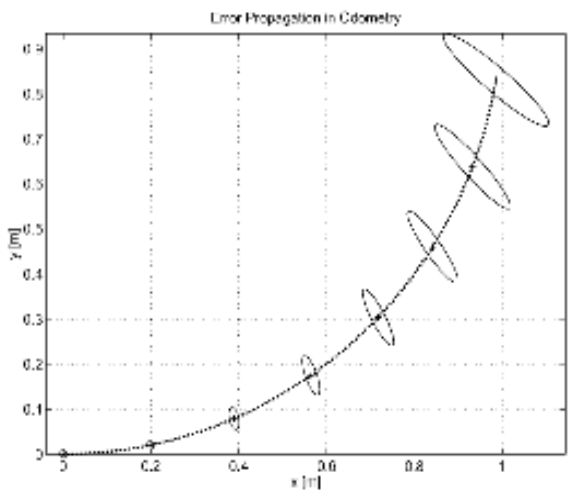
\includegraphics[width=0.6\textwidth]{poseUncertainity.png}
    \attribution{R. Siegwart, I.R. Nourbakhsh, Introduction to Autonomous Mobile Robots}
\end{center}

Видно, что неопределённость касательно направления робота растёт быстрее, чем неопределённость поступательного движения (что в целом неудивительно, небольшое отклонение в скорости вращения одного из колёс заставит робот сильнее заворачивать в сторону и с течением времени уехать сильно вбок, тогда как чтобы накапливать ошибку поступательного движения, роботу надо постоянно двигаться быстрее или медленнее заданной скорости).
Ещё видно, что ось эллипса неуверенности в позе не перпендикулярна истинной траектории (что тоже понятно чисто по геометрическим соображениям --- по малому кругу путь короче, чем по большому).

Поэтому при работе с датчиками возникают важные соображения:

\begin{itemize}
    \item \emph{при работе с датчиками всегда-всегда используется фильтрация} --- это может быть какой-то простой фильтр типа скользящего среднего, медианный фильтр, или что-то более продвинутое типа фильтра Калмана;
    \item неопределённость --- это нормально, с ней надо уметь работать, в частности, всегда представлять оцениваемые по показаниям датчиков параметры как случайную величину;
    \begin{itemize}
        \item при этом если мы ожидаем только случайные ошибки, можно использовать представление неопределённости с одной гипотезой, если может быть систематическая ошибка, алиасинг и т.п., то имеет смысл использовать представление с несколькими гипотезами (например, как случайную величину с мультимодальным распределением); 
            с несколькими гипотезами одновременно работать гораздо сложнее, поскольку каждую гипотезу надо обновлять при получении новых показаний, некоторые гипотезы будут \enquote{умирать}, некоторые, наоборот, \enquote{разветвляться};
    \end{itemize}
    \item надо уметь сливать показания нескольких сенсоров в одно (sensor fusion) --- например, если на роботе установлены лидар и стереокамера, можно получить гораздо более точные показания и устранить некоторые систематические ошибки, корректируя один датчик по показаниям другого;
        однако это не так просто, как кажется, для этого тоже требуется продвинутая математика и иногда даже машинное обучение.
\end{itemize}

\subsection{\enquote{Высокоуровневая} сенсорика}

Самые информативные датчики на роботе --- это камеры, поэтому машинному зрению в робототехнике уделяется особенное внимание. Вот что можно получить по видео.

\begin{itemize}
    \item Depth from focus --- простой (относительно) способ измерения расстояния до объекта, если камера позволяет изменять фокусное расстояние.
        Меняем фокусное расстояние до тех пор, пока изображение не становится резким (резкость можно посчитать с помощью некоего матана, называемого \emph{градиентом интенсивности}), зная текущее фокусное расстояние и параметры камеры можно посчитать расстояние до объекта в фокусе.
        Проблема в том, что честно менять фокусное расстояние можно только механически (всякие программные вещи типа повышения резкости, используемые, например, в смартфонах, тут, понятно, бесполезны), а это сложная механика, поэтому дорого и на самых распространённых камерах такого не бывает (разве что вручную объектив крутить, но для роботов это такое себе решение).
    \item Feature-based-стерео --- это на самом деле много разных алгоритмов сопоставления точек на кадрах с разных ракурсов. Принцип действия такой, что мы берём две камеры, делаем одновременно обеими снимок одной сцены, сравниваем два снимка, находим одинаковые точки на изображениях (может и не одинаковые, но соответствующие одной точке на сцене), и, зная расстояние между камерами (\emph{базу} стереопары), триангуляцией получаем расстояние до точки.
        Даже до всех точек в кадре, для которых однозначно нашлась пара.
        Чтобы облегчить процесс поиска пар точек, для каждой точки на изображении строится \emph{дескриптор} --- некое характерное представление точки, не зависящее от ракурса.
        Обычно дескрипторы считаются по соседним точкам и достаточно быстро, в результате чего по каждой точке получаем число, сортируем массивы этих чисел и ищем совпадения на левом и правом изображении.
        Дальше считаем, что нашли пары, но поскольку дескрипторы могут совпасть чисто случайно (они сродни хеш-функции), надо ещё пройтись по изображениям и проверить, что геометрически близким точкам на одном изображении соответствуют геометрически близкие точки на втором, а все точки, для которых это не так, выкинуть из сопоставления.
        Однозначно сопоставить точки с помощью дескрипторов можно только если они чем-то отличаются от остальных --- такие точки называют характерными точками (feature points), и померить расстояние можно только до них.
        Если на изображении нет характерных точек (оно монотонно или имеет повторяющуюся текстуру), стерео работать не будет.

        Дьявол, разумеется, кроется в деталях --- как считать дескрипторы, можно ли их вообще не считать (бывают алгоритмы глобального сопоставления), как фильтровать результаты и т.п.

        И ещё внезапно оказывается, что двух камер для стереопары и не надо --- одной камеры и возможности сколько-нибудь точно узнать пройденное роботом расстояние (например, с помощью энкодеров) достаточно, чтобы сделать стереопару.
        Получится хуже, чем настоящая стереопара (точное положение робота не посчитать, плюс два снимка не синхронны, поэтому сцена могла успеть измениться и правильно сопоставить точки не выйдет), зато бюджетно.
        Так работает, например, ORB SLAM.
        Настоящая стереопара, кстати, это не просто две камеры, \enquote{прибитые} к одной планке --- они ещё, как правило, аппаратно синхронизируют время съёмки. 
    \item Оптический поток --- имея два кадра в разные моменты времени, можно искать движение.
        В основном это делается тоже поиском характерных точек и их сопоставлением между кадрами, но уже без требования \enquote{локальности} сопоставленных точек.
        Просто обнаружить движение можно ещё проще --- сделать последовательно два кадра и вычесть один из другого (прямо вот арифметически), где получится не ноль (сильно не ноль --- надо сделать поправку на шумы и изменение освещённости) --- там было движение.
        Однако честно считать оптический поток информативнее, поскольку можно получить скорость движущегося объекта.
        А если движется не объект на сцене, а мы, оптический поток может позволить нам оценить нашу собственную скорость --- это называется \enquote{визуальная одометрия}.
    \item Поиск границ, поиск геометрических примитивов --- есть довольно простые методы, позволяющие вычленить на изображении структурные элементы.
        Границы контуров на изображении можно найти с помощью лапласиана гауссиана или несколько более продвинутого оператора Кэнни.
        Звучит сложно, но на самом деле это просто \sout{свёртка с ядром} умножение числовых значений пикселей на изображении на некую матрицу (мы кусочек изображения рассматриваем как матрицу 3 на 3 или 5 на 5 и умножаем на матрицу линейного оператора, получая преобразованное изображение, где остались только контуры).
        
        Искать прямые линии тоже довольно просто, с помощью несколько менее тривиальной, но красивой идеи --- преобразования Хафа.
        Идея его в том, что каждая точка изображения \enquote{голосует} за параметры прямых, которые через неё проходят (в пространстве Хафа прямая описывается двумя параметрами --- расстоянием от центра координат и углом наклона), и за какие параметры проголосовало больше точек, те и соответствуют прямым на изображении:

        \begin{center}
            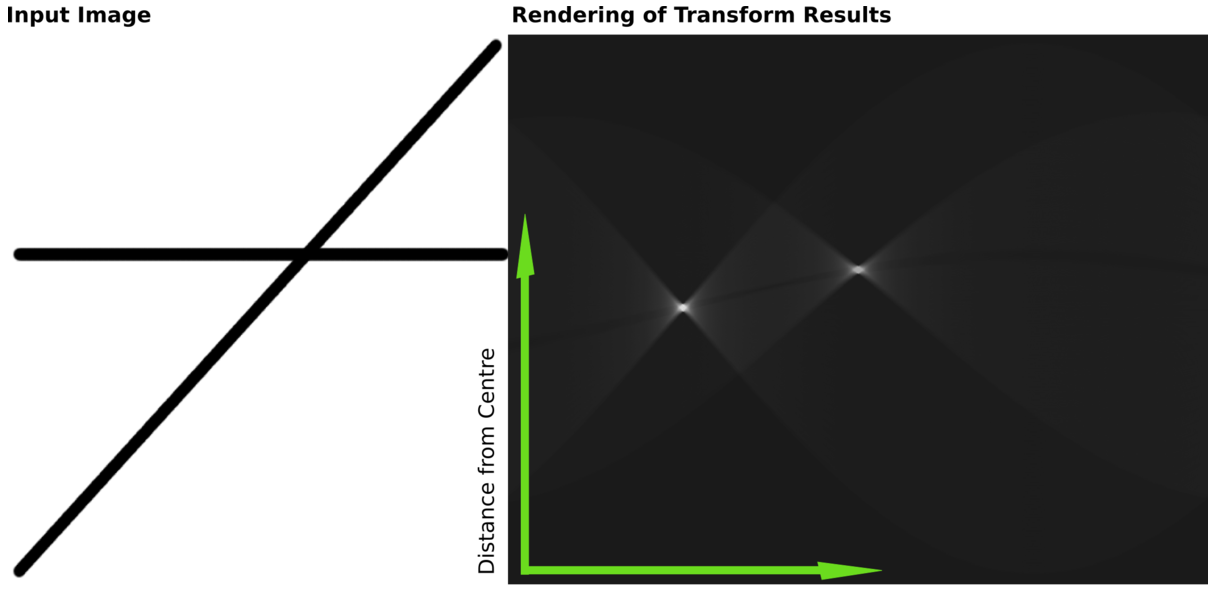
\includegraphics[width=0.7\textwidth]{houghTransform.png}
            \attribution{\url{https://ru.wikipedia.org/wiki/Преобразование_Хафа}}
        \end{center}

        Алгоритм Хафа обобщается и на окружности, и на другие геометрические примитивы.

    \item Сегментация, кластеризация --- изображение можно разбить на области, про которые сказать, что вот это дерево, это автомобиль, это пешеход. 
        Или кластеризовать похожие точки, например, собрав их в плоскость, или в линию дорожной разметки.
        В этом деле могут помочь некоторые классические алгоритмы, такие как DBSCAN и RANSAC, но более популярны методы машинного обучения.
        Впрочем, в робототехнике они не всегда применимы в силу ограниченности бортовых вычислительных мощностей, желания экономить аккумулятор и действия без широкополосного интернет-соединения.

    \item Whole-image features --- более простые методы, позволяющие понять, достигли ли мы цели, или искать текущее изображение в базе.
        Это, например, цветовые гистограммы --- когда мы цвета пикселей раскладываем по корзинам гистограммы и получаем более-менее уникальный для изображения вектор частот цветов.
        \enquote{Отпечатки} изображений --- это в общем случае способ построить какую-то характеристику изображения, которая компактнее и проще самого изображения, но при этом достаточно уникальна.
        Если робот должен оказаться в какой-то комнате, может быть хорошей идеей сделать панорамный снимок окружения и сравнить его с заранее посчитанным отпечатком целевой комнаты.
        Или если мы сфотографировали здание, можем сегментировать здание, посчитать отпечаток для сегмента и сравнить с базой отпечатков, чтобы понять, что это за здание.
\end{itemize}

Общая схема высокоуровневой сенсорики на компьютерном зрении и используемые при этом инструменты выглядят вот так:

\begin{center}
    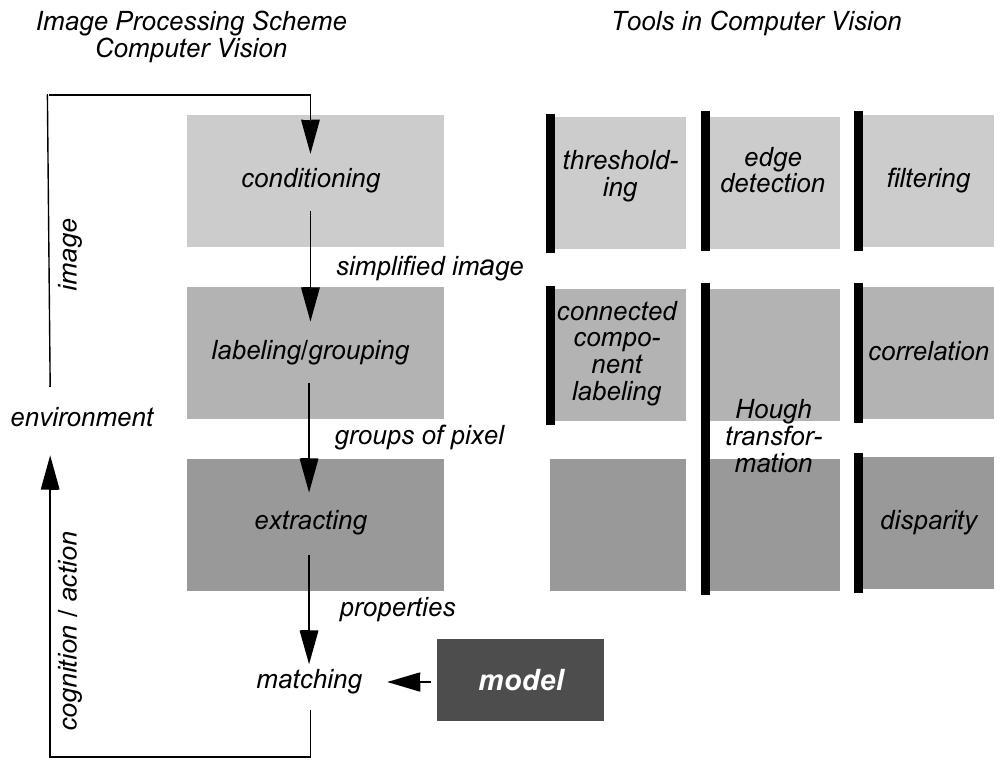
\includegraphics[width=0.8\textwidth]{cvScheme.png}
    \attribution{R. Siegwart, I.R. Nourbakhsh, Introduction to Autonomous Mobile Robots}
\end{center}

Первая фаза --- это предобработка изображения: фильтрация, нормализация яркости, перевод в \enquote{правильное} цветовое пространство и т.п.
Затем --- кластеризация или группировка в том или ином виде, будь то семантическая сегментация, выделение контуров и т.п.
Затем выделение интересных характеристик, например, распознавание дорожного знака.

В качестве основного инструмента сейчас используются различные нейронные сети, но по сути они часто пытаются аппроксимировать классические алгоритмы, перечисленные справа.
Не всё можно делать нейросетями --- как из соображений потребных вычислительных мощностей, так и из-за более странных причин.
Например, в сфере беспилотных автомобилей законодательно нельзя использовать неинтерпретируемые методы --- то есть всегда должно быть можно объяснить, почему автомобиль повёл себя именно так.
Нейросети таким свойством не обладают, поэтому в этой сфере играют лишь вспомогательную роль, предпочтение отдаётся интерпретируемым методам типа деревьев решений.

\section{Локализация}

Теперь, когда мы с помощью датчиков более-менее умеем анализировать мир вокруг, возникает задача поиска пути до целевой точки.

Вообще, задача навигации решается двумя способами.

Поведенческая (или реактивная) навигация: 

\begin{center}
    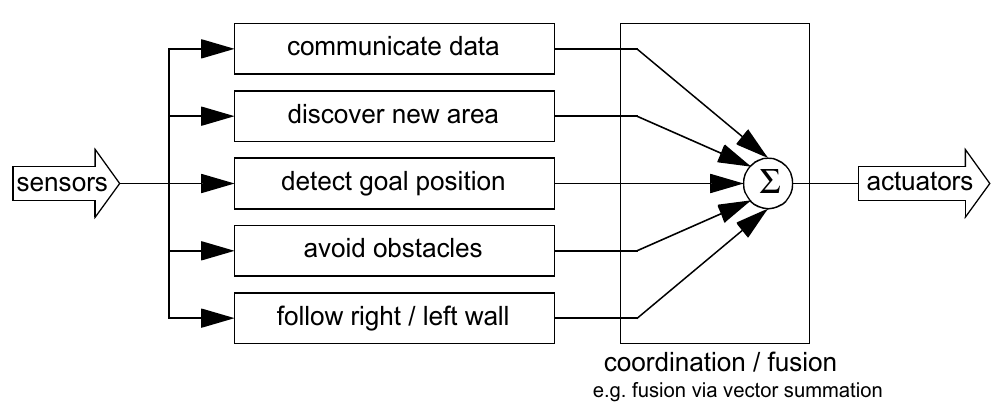
\includegraphics[width=0.65\textwidth]{behaviorNavigation.png}
    \attribution{R. Siegwart, I.R. Nourbakhsh, Introduction to Autonomous Mobile Robots}
\end{center}

--- едем пока можем, особо не важно куда, избегая препятствий, пока не окажемся в искомой точке.
Идеально работает, если мы ничего не знаем об окружающем пространстве или точке назначения --- например, при действиях в быстро изменяющемся окружении.

Навигация по карте:

\begin{center}
    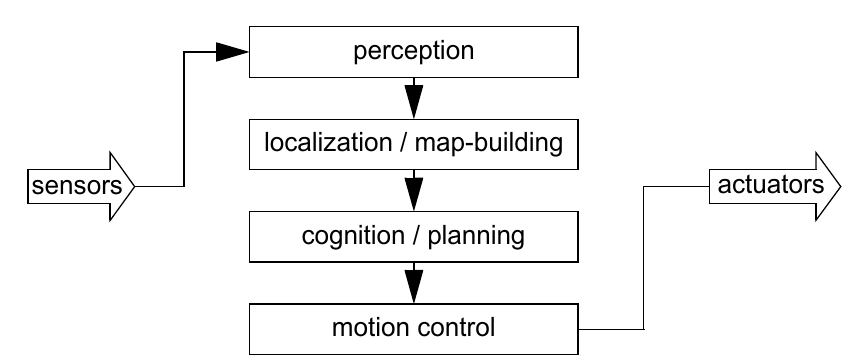
\includegraphics[width=0.6\textwidth]{mapBasedNavigation.png}
    \attribution{R. Siegwart, I.R. Nourbakhsh, Introduction to Autonomous Mobile Robots}
\end{center}

Либо у нас есть заранее известная карта и мы по данным сенсоров локализуемся, планируем действия, строим маршрут и потом его исполняем, либо карта заранее неизвестна и мы строим её в процессе работы, планируя и строя маршрут на уже известном участке карты (возможно, так, чтобы эффективно исследовать неизвестные).
Подход с картой гораздо сложнее в реализации, чем поведенческий, плюс требует немалых ресурсов на хранение карты, но может быть гораздо полезней.

\subsection{Представление неточности локализации}

Итак, до того, как заниматься навигацией, надо локализоваться.
А для того, чтобы локализоваться, надо понять, что будет результатом локализации.
К этому моменту уже должно быть понятно, что задача локализации не состоит в определении позы робота относительно глобальной системы координат, поскольку в условиях шумов и систематических ошибок датчиков эта задача нерешаема.
А ещё есть алиасинг.

Простой пример:

\begin{center}
    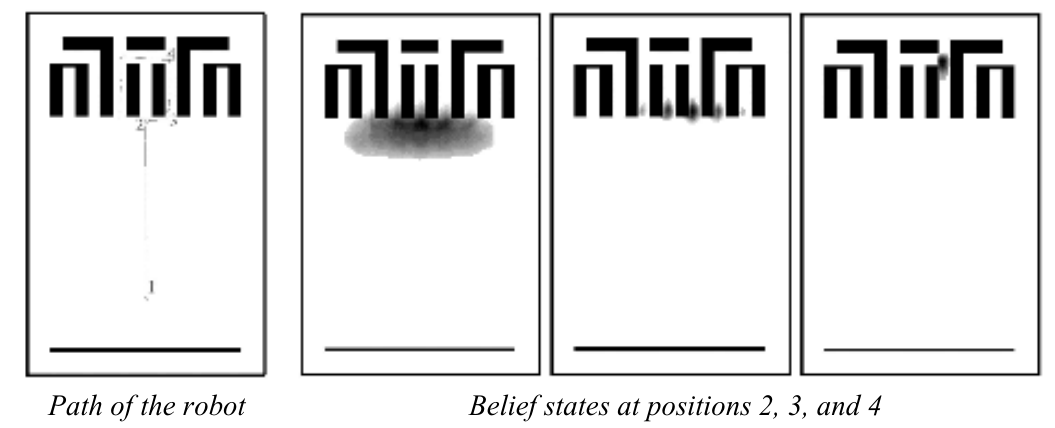
\includegraphics[width=0.9\textwidth]{uncertainity.png}
    \attribution{R. Siegwart, I.R. Nourbakhsh, Introduction to Autonomous Mobile Robots}
\end{center}

На картинке не рассмотреть путь робота (по историческим причинам), но идея понятна --- зная только показания датчиков, которые \enquote{видят} на некотором ограниченном расстоянии, мы не можем точно сказать, где находимся.
Подъезжая к нижней части района препятствий мы наблюдаем отрытые пространства, чередующиеся с препятствиями --- на данной карте они все одинаковы, так что ориентироваться мы можем только на одометрию.
Поскольку одометрия принципиально неточна, наше представление о текущей позиции весьма размыто --- мы точно не у краёв карты (вряд ли мы могли так ошибиться), но в какой именно из проходов мы заезжаем, мы без идей.

Двигаясь по проходу, мы можем уточнить свою позицию как одну из пяти возможностей, причём с разными вероятностями (за счёт данных одометрии) --- мы скорее всего движемся где-то по центру, но могли сместиться влево-вправо.

Доехав до отворота влево мы можем наконец относительно точно локализоваться --- на карте больше нет мест, где справа стена, а слева и спереди свободно.
Почему относительно --- мы знаем, на каком мы перекрёстке, но не знаем, где именно --- датчики ведь врут.

В данном случае представлять позицию робота надо было с помощью смеси нормальных распределений, каждый элемент которой оценивался независимо и отвергался либо уточнялся в зависимости от показаний датчиков. В общем случае представлять знания робота о позиции можно четырьмя способами:

\begin{center}
    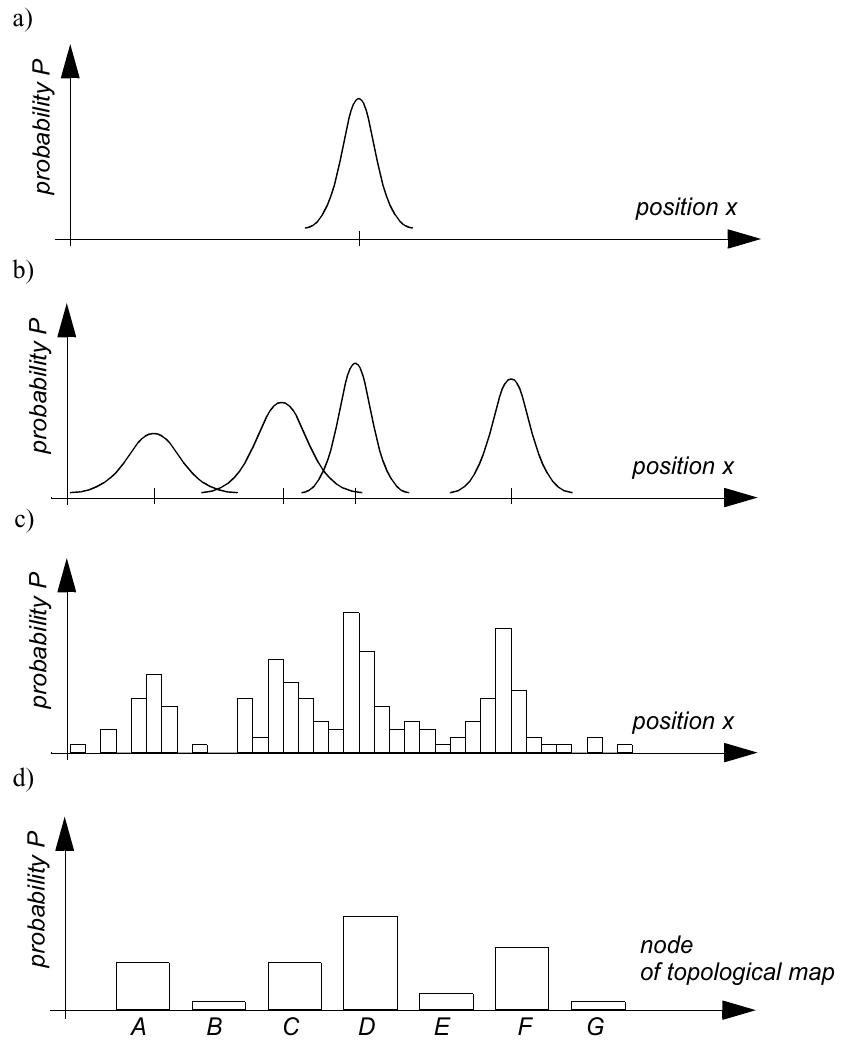
\includegraphics[width=0.5\textwidth]{beliefRepresentation.png}
    \attribution{R. Siegwart, I.R. Nourbakhsh, Introduction to Autonomous Mobile Robots}
\end{center}

\begin{enumerate}
    \renewcommand{\labelenumi}{\alph{enumi}}
    \item \enquote{Обычное} (одномодальное) нормальное распределение для непрерывных координат робота.
    \item Мультимодальное нормальное распределение в непрерывном случае (как в примере выше).
    \item Дискретное мультимодальное распределение для клеточной карты --- тут хранится вероятность, в которой робот находится в той или иной ячейке.
    \item Дискретное распределение для топологической карты --- тут для каждого узла графа, которым представляется карта, хранится вероятность, что робот в этом узле.
\end{enumerate}

Кстати, \enquote{Знания робота} в роботехнике говорят, говорят \enquote{Представления робота} (или, лучше, по-английски, \foreignquote{english}{Beliefs}, \enquote{Верования}) --- робот не может знать наверняка, он может только верить в то, что он в такой-то позиции.
Это же касается и всех остальных знаний робота о внешнем мире, включая не относящиеся к навигации данные типа температуры.
Есть значения с датчиков, которые являются выборкой некоей случайной величины с возможной систематической ошибкой, по ним строится некое представление, которое потом уточняется с помощью процесса сбора и анализа дополнительных сведений (или, по-английски, \foreignquote{english}{Evidence accumulation}), в ходе которого часть гипотез отвергается, часть уточняется.

\subsection{Представление карты}

Выше зашла речь про локализацию в непрерывном пространстве, клеточную карту и странную вещь --- топологическую карту.
Дело в том, что как именно хранить карту --- тоже важное архитектурное решение.
Концептуально подходов два --- непрерывный и дискретный.

В непрерывном представлении карта хранится как набор геометрических примитивов, которые либо заранее известны, либо выделяются роботом в процессе исследования окружения.
Например, преобразованием Хафа из данных дальнометрии можно выделить линии --- границы препятствий, которые потом эффективно хранить в памяти.

В дискретном представлении пространство делится на сетку, каждая ячейка может быть либо препятствием, либо открытым пространством.
Например, реальные препятствия могут быть дискретизированы по правилу \enquote{если в клетке есть хоть какая-то часть препятствия, клетка считается непроходимой}:

\begin{center}
    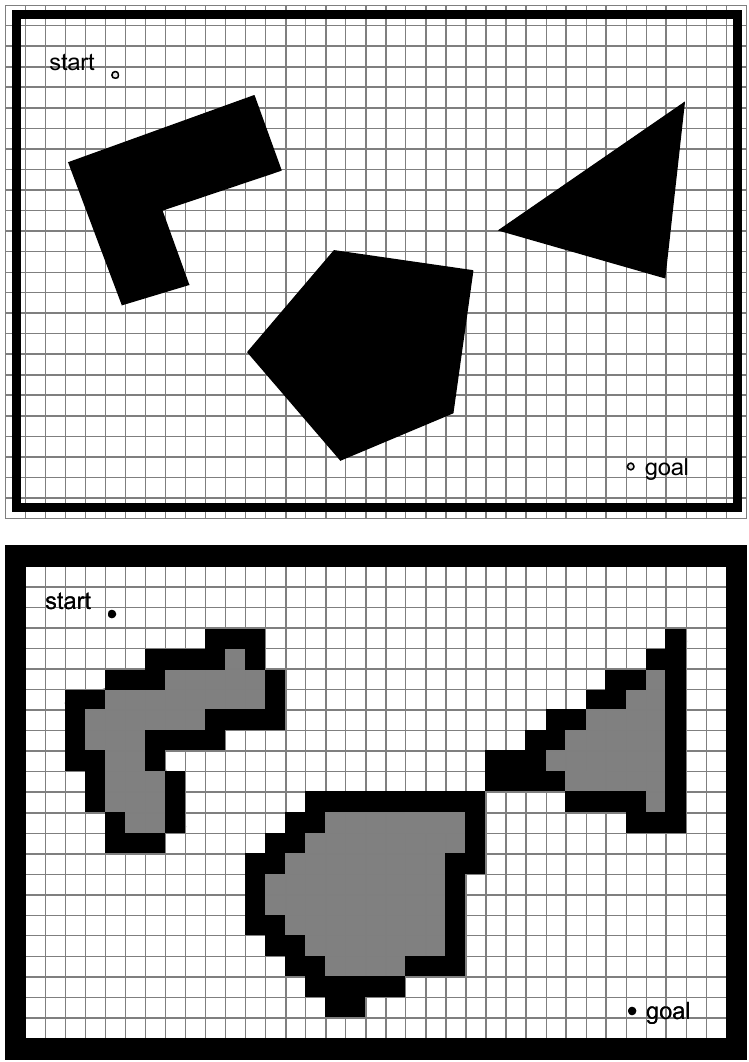
\includegraphics[width=0.5\textwidth]{fixedCellGrid.png}
    \attribution{R. Siegwart, I.R. Nourbakhsh, Introduction to Autonomous Mobile Robots}
\end{center}

Такой подход прост, но не очень эффективен в плане памяти, и склонен к артефактам (тут мы видим, что проход между двумя препятствиями справа представляется как непроходимый).

Несколько более сложно, но более интересно хранить карту в представлении, напоминающем дерево квадрантов:

\begin{center}
    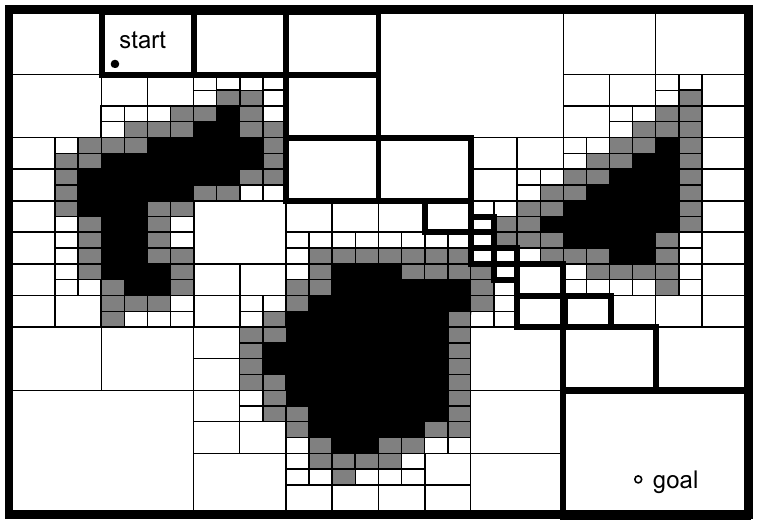
\includegraphics[width=0.5\textwidth]{variableCellGrid.png}
    \attribution{R. Siegwart, I.R. Nourbakhsh, Introduction to Autonomous Mobile Robots}
\end{center}

Границы препятствий уточняются мелкими клетками, области, в которых ничего интересного не происходит, представляются крупными.

Ну и самый радикальный способ --- это вообще не хранить границы препятствий, поднявшись на уровень выше (и надеясь на behavior-driven-подход к локальной навигации):

\begin{center}
    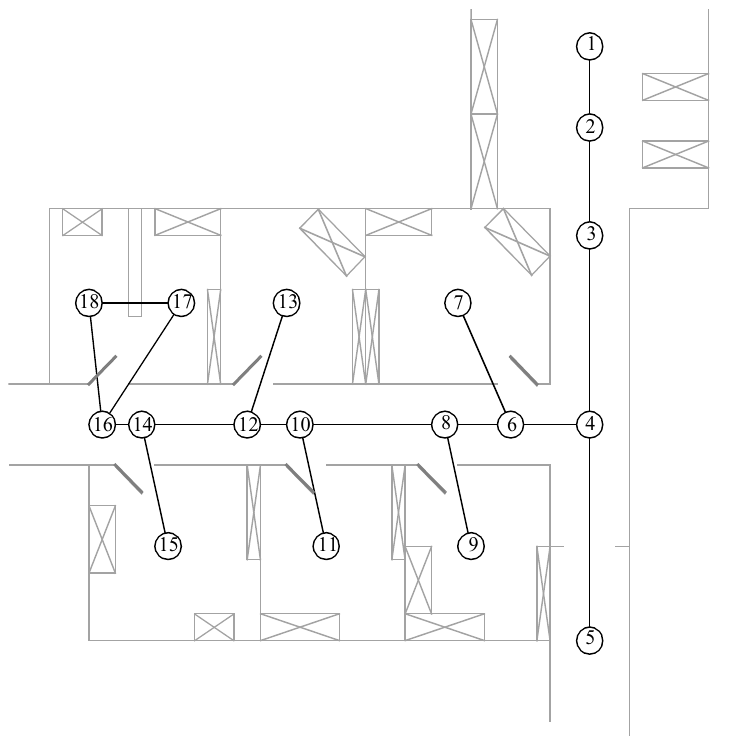
\includegraphics[width=0.7\textwidth]{topologicalMap.png}
    \attribution{R. Siegwart, I.R. Nourbakhsh, Introduction to Autonomous Mobile Robots}
\end{center}

Такая карта хранит просто информацию о связности между интересными зонами (тут --- комнатами), по ней можно строить путь, можно локализоваться с точностью до зоны, это эффективно по памяти, просто, и зачастую вполне достаточно для прикладных задач.
Но, конечно, неточно, и может приводить к неоптимальным в плане поиска пути решениям --- робот с честной картой поедет по кратчайшему пути, робот с топологической картой --- к центру комнаты, или будет метаться вдоль стенок.

\subsection{Подходы к локализации}

Итак, мы выбрали представление карты, научились представлять на ней положение робота, теперь наша задача --- собственно, определять это положение с наибольшей возможной точностью (собственно, \emph{локализация}).
Тут возможно несколько подходов.

\begin{itemize}
    \item Инерциальная навигация, проприоцепция.
        \emph{Проприоцепция}, в противоположность \emph{экстероцепции} --- внутреннее ощущение положения в пространстве, без внешних ориентиров.
        В роботах бывает за счёт энкодеров и акселерометров --- они измеряют, что происходит с роботом, а не что происходит с миром вокруг.
        Инерциальная навигация --- частный случай проприоцепции, использующий акселерометр и датчики угловых скоростей.
        Навигация по энкодерам --- одометрия.
        Как мы видели выше, хорошо работает на коротких дистанциях и временных промежутках, если нет другого способа навигации.
        Требует внешней коррекции вне \enquote{эпсилон-окрестности} начальной точки.
    \item Локализация по ориентирам --- когда у нас есть координаты в глобальной системе координат некоторых ориентиров и возможность локализоваться относительно них.
        Например, спутниковая навигация, навигация по маякам, тэгам или визуальным ориентирам.
        Поскольку локализоваться относительно ориентира мы можем только с помощью датчиков, а датчики врут и бывает алиасинг, используются методы представления неопределённости и уточнения гипотез:
    \begin{itemize}
        \item марковская локализация --- поддерживаем набор предположений о том, где мы, и уточняем по показаниям сенсоров;
        \item локализация на основе фильтра Калмана --- решаем математическую задачу оптимизации предсказанного положения робота и данных сенсоров.
            Вот принципиальная схема локализации с фильтром Калмана:
            \begin{center}
                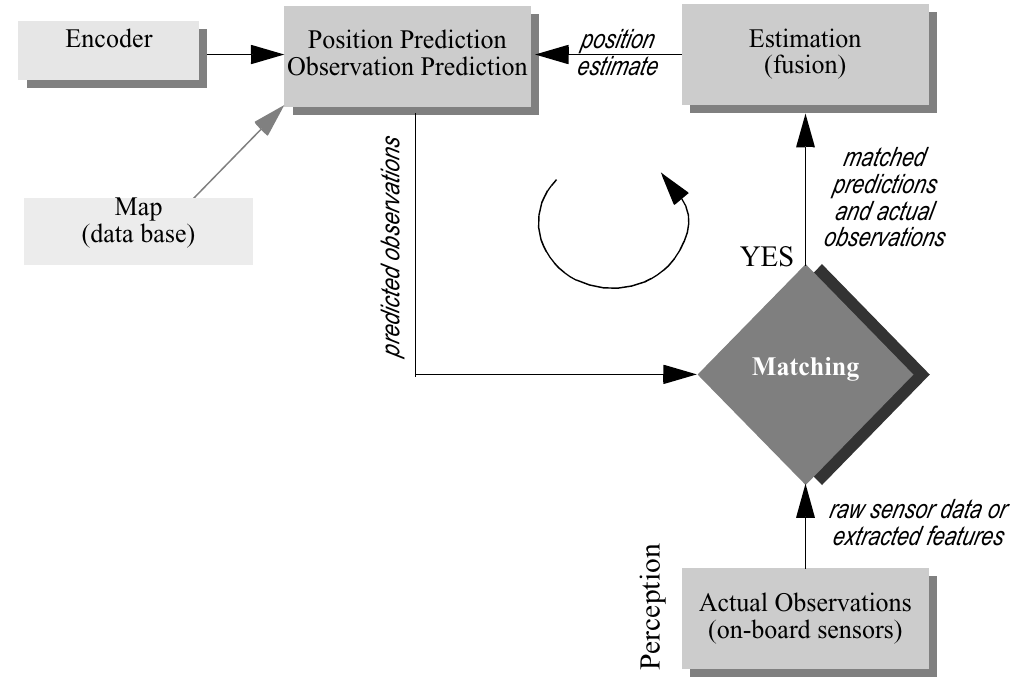
\includegraphics[width=0.7\textwidth]{kalmanLocalization.png}
                \attribution{R. Siegwart, I.R. Nourbakhsh, Introduction to Autonomous Mobile Robots}
            \end{center}
    \end{itemize}
    \item Simultaneous Localization And Mapping (SLAM) --- это когда мы строим карту и пытаемся определить своё положение на ней.
        Применяется, когда карта заранее неизвестна, или цель робота и состоит в её построении.
        Вот принципиальная схема работы SLAM:
        \begin{center}
            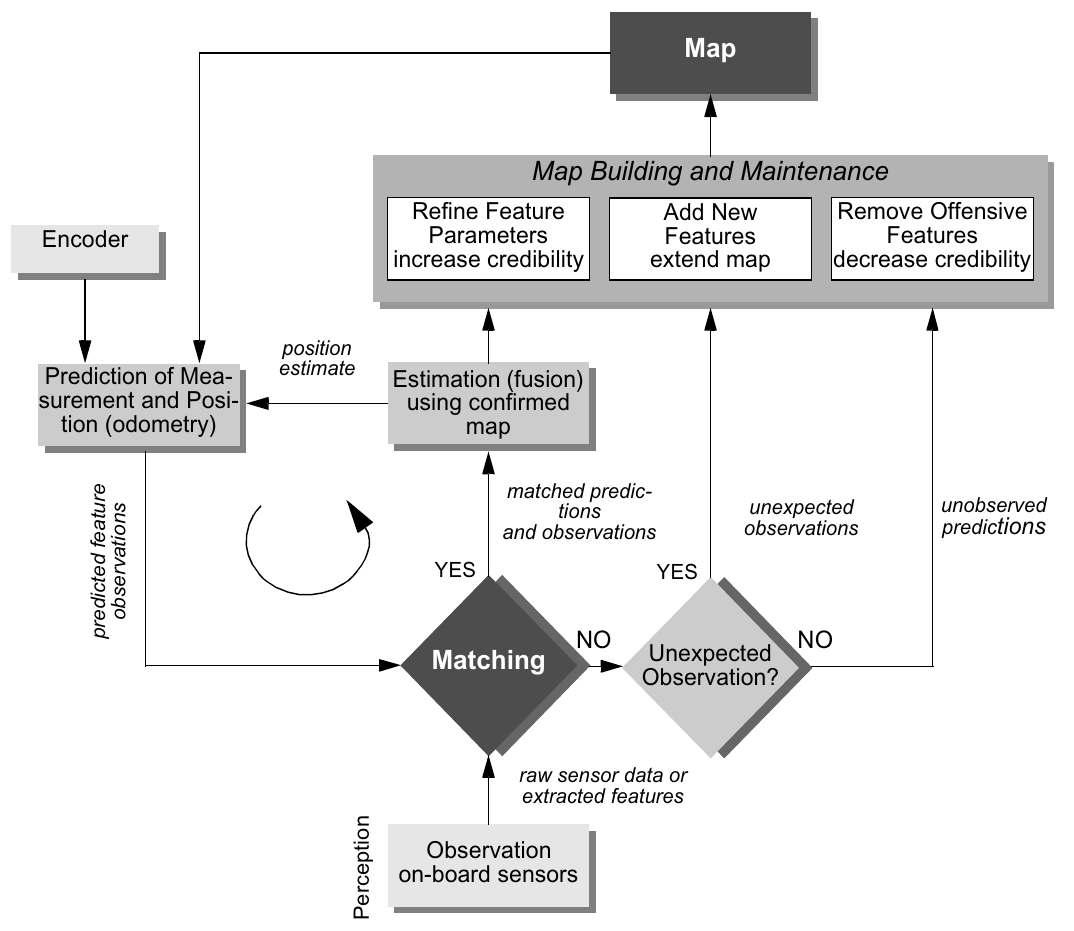
\includegraphics[width=0.7\textwidth]{slam.png}
            \attribution{R. Siegwart, I.R. Nourbakhsh, Introduction to Autonomous Mobile Robots}
        \end{center}
\end{itemize}

SLAM на самом деле очень распространённый и перспективный метод локализации, всё-таки он не требует исходной карты.
Однако ввиду накопления ошибки наивная реализация SLAM может привести к ряду занятных проблем, таких как, например, \emph{замыкание цикла}:

\begin{center}
    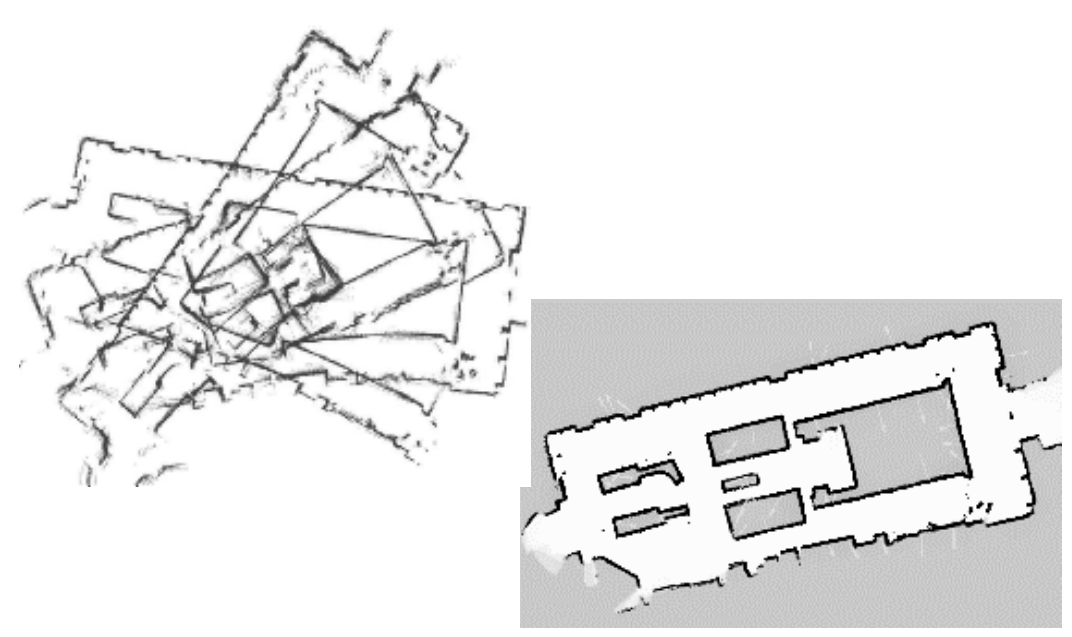
\includegraphics[width=0.7\textwidth]{slamErrors.png}
    \attribution{R. Siegwart, I.R. Nourbakhsh, Introduction to Autonomous Mobile Robots}
\end{center}

Проблема замыкания цикла состоит в том, что робот, двигаясь по циклической траектории, должен попасть в точку старта, получив согласованное представление о карте мира вокруг.
Однако из-за ошибок позиционирования, которые имеют свойство накапливаться, карта начинает \emph{сползать} и в итоге получается что-то с самопересечениями и совсем не соответствующее истине.
Чинится это корректировкой позиции робота по уже имеющимся картографическим данным (\emph{топологическая коррекция}) --- мы ожидаем, что ориентиры в окружающем пространстве останутся на своём месте, прямые будут прямыми и т.п., поэтому можем на самом деле уточнить позицию робота.

\section{Навигация}

Наконец, предельно кратко про последний этап цикла \enquote{Sense-Compute-Control} --- построение пути и движение по траектории.

Задача навигации --- зная карту и своё положение на ней, достичь позиции (или группы позиций) $p$ в момент времени не позже некоего $n$.
Однако понятно, что мы не знаем своё положение, поэтому не можем знать, достигли мы заданной позиции $p$ или нет.
Поэтому задача навигации на самом деле формулируется так --- зная свои текущие представления о текущем состоянии карты (она ведь может меняться!) и своё представление о положении на ней, достичь состояния, в котором мы верим, что достигли позиции (или группы позиций) $p$ в момент времени не позже некоего $n$.

Поэтому принимается за данное, что мы в процессе движения по проложенной траектории можем уточнять наши знания о мире, обнаруживать и избегать движущихся препятствий, поэтому обычно говорят не о задаче навигации, а об интегрированном планировании и исполнении пути (\enquote{integrated planning and execution}).

Однако проблема в том, что поиск маршрута --- это не просто прогнать Дейкстру по графу, это, в общем случае, решение задачи обратной кинематики робота при наличии кучи ограничений.
Это небыстро.
А управление на моторы надо подавать в реальном времени. 
Поэтому типовая архитектура для систем управления --- слоистая, где каждый слой работает параллельно, циклично, с разной частотой одного цикла:

\begin{center}
    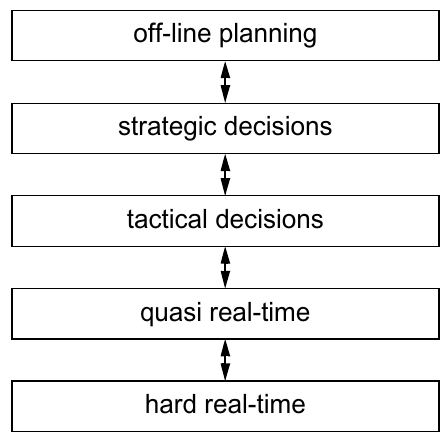
\includegraphics[width=0.4\textwidth]{navigationLayers.png}
\end{center}

В самом низу находятся контроллеры моторов, они часто реализуются аппаратно, хотя возможны варианты.
Их работа --- генерация \emph{ШИМ}-сигнала на мотор.
ШИМ, или широтно-импульсная модуляция (PWM по-английски) --- это способ управлять оборотами электромотора. 
На электромотор можно было бы подавать меньшее напряжение, но обычно напряжение в цепи питания фиксировано, и моторы перепадов напряжения не любят, поэтому используется приём, когда часть времени на мотор подаётся полное напряжение, часть --- напряжение не подаётся вовсе.
Суммарная мощность, а следовательно и обороты мотора, определяются соотношением зон с подачей напряжения и зон без подачи, а отсутствие дёрганий достигается за счёт частых переключений, чтобы инерция ротора мотора создавала непрерывное вращение с примерно одинаковой угловой скоростью.
ШИМ вполне можно генерировать программно, но это надо делать в реальном времени (иначе мотор будет дёргаться или вообще встанет).
Поэтому часто этим занимаются контроллеры (или \emph{драйверы}) моторов, которые принимают во входные регистры параметры ШИМ-сигнала, и в реальном времени генерируют его на выход.
При этом выходное напряжение драйвера может быть гораздо больше используемого центральным процессором робота, что позволяет обычными платами управлять сколь угодно мощными моторами через драйвер.

Слой выше решает вопросы избежания столкновений и аварийного останова робота.
Это надо делать в настолько реальном времени, насколько возможно, хотя уже требует некоторых продвинутых алгоритмов и опроса датчиков (которые в принципе не могут отвечать мгновенно), поэтому уж как получится.
Тем не менее, реализация аварийного останова может быть критичной для безопасной эксплуатации робота.

На этом же слое может работать код опроса датчиков.
Опрос датчиков нет смысла делать честно внутри цикла \enquote{sense-compute-control}, поскольку работа датчиков требует времени, зачастую немалого, что затрудняет управление временем для управления --- а ведь выработка управляющего воздействия должна вестись в соответствии с математической моделью, раз в строго определённый временной промежуток.
Опрос идёт в квазиреальном времени постоянно, данные сохраняются в регистрах или памяти, и предоставляются по запросу.

Слои выше отвечают за планирование с различной степенью гранулярности и различной скоростью работы.
Например, оффлайн-планирование может вообще не выполняться на борту, а загружаться в робот при старте миссии.
Исходя из него робот иногда оценивает ситуацию и принимает стратегические решения (например, в какую комнату ехать), а исходя из стратегических решений выполняется тактическое планирование (например, прокладка маршрута).
Тактическое планирование может перезапускаться очень часто в силу изменчивости внешнего мира.

Вот пример такой архитектуры:

\begin{center}
    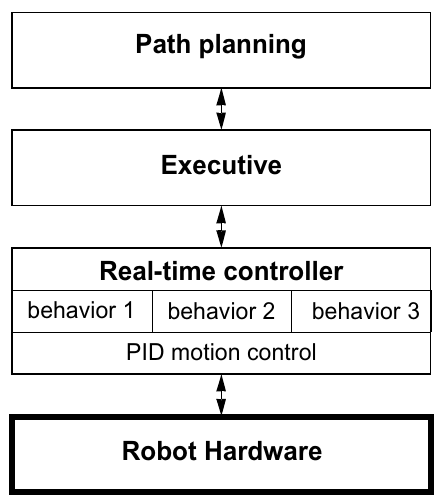
\includegraphics[width=0.35\textwidth]{navigationTiers.png}
\end{center}

Аппаратное обеспечение подчиняется ПИД-регулятору, работающему в реальном времени, который, в свою очередь, параметризуется разными работающими параллельно поведениями (движение к цели, избежание препятствий и т.п.).
Задачи поведениям ставит исполнительная часть, реализующая кинематическую модель робота, а е в свою очередь ставит задачи навигационная подсистема, прокладывающая путь.

\section{Программно-инженерные аспекты}

Теперь, совсем наконец, поговорим о том, как и на чём это всё реализуют.

Разработка робота ведётся в соответствии с его математической моделью и зачастую параллельно с её проработкой.
Чем больше возможности \enquote{железа} робота, тем менее сложной может быть математическая модель --- например, если вычислительные возможности позволяют обсчитывать управление за наносекунды, временем дискретизации практически можно пренебречь, а если датчики очень точны, то пренебречь шумами.
Однако если оборудование далеко от идеала (а значит, дёшево и распространено), то матмодель должна это учитывать --- появляются всякие интересные с теоретической точки зрения вещи типа \emph{управления с запаздыванием}, про которые до сих пор защищают диссертации, несмотря на то, что кибернетике уже очень много лет.

Разработка чаще всего ведётся по V-образной модели с активным использованием имитационного моделирования --- требования, затем математическая модель, затем алгоритмы, отладка на симуляторе, выбор аппаратной платформы, реализация \emph{в железе}, отладка, апробация.
На каждом этапе что-то может пойти не так, происходит откат на соответствующий этап V-образной модели разработки --- особенности \emph{железа} могут потребовать корректировки математической модели, результаты испытаний --- требований и т.п.
Важно использование симуляторов, поскольку, в отличие от разработки обычного программного обеспечения, киберфизическую систему довольно легко привести в негодность, тысячей различных способов.
Поэтому сначала всё программное обеспечение тестируют в симулируемом окружении, потом на реальном роботе.

Какой сейчас есть выбор аппаратных платформ:

\begin{itemize}
    \item готовые роботы --- это прежде всего роботы-манипуляторы KUKA, они дороги, но свой робот-манипулятор с адекватной точностью собрать практически без шансов;
    \item платы \enquote{сделай сам} --- прежде всего, сейчас это Arduino в различных вариациях, или для вычислительно сложных задач типа машинного зрения или машинного обучения --- Raspberry Pi; 
        есть и более новые, модные и перспективные платформы, типа MIK32 АМУР или НИИЭТ К1921ВГ015 на ядре RISC-V --- открытая архитектура, крайне низкое энергопотребление и достаточная производительность (плюс куча периферии на кристалле, вплоть до встроенной поддержки автомобильной шины CAN) делают их очень привлекательными для робототехники; опять же, импортозамещение --- два последних микроконтроллера делаются в России;
        проблема \enquote{голых} плат в том, что периферию типа драйверов моторов или датчиков к ним надо буквально припаивать паяльником, а потом ещё и программировать на странных диалектах Си;
    \item образовательные платформы, платформы для прототипирования --- прежде всего, ТРИК. Он создавался как достаточно производительный контроллер с большим числом портов для периферии, чтобы применяться для быстрой сборки прототипов, и только потом пошёл в образовательную сферу. Есть ещё Vex и Fishertechnik --- это тоже \enquote{продвинутые} образовательные наборы, которые даже взрослые робототехники используют, чтобы быстро что-то собрать и попробовать.
\end{itemize}

Симуляторы:

\begin{itemize}
    \item Player/Stage/Gazebo --- некогда стандарт де-факто в робототехнических исследованиях, умеет сносно симулировать сцену, физику, датчики и т.п., очень расширяем (на самом деле это набор инструментов), очень старый и зрелый, но страшный как моя жизнь, поэтому нынче вышел из моды --- со смещением фокуса в робототехнике на машинное зрение управлять цветными параллелепипедами на клетчатом полу уже не так интересно;
    \item Webots --- тоже старый, но выглядящий более прилично, чем Gazebo, симулятор, хорошо поддерживает группы роботов, прост в обращении, поэтому любим в лабораториях СПбГУ;
    \item CoppeliaSim (бывший V-REP) --- тоже достойный симулятор, мы как-то делали интеграцию с ним для среды TRIK Studio;
    \item Microsoft AirSim --- изначально создавался для исследований в области искусственного интеллекта для БПЛА, теперь поддерживает и наземные роботы, хорош набором инструментов для машинного зрения --- симуляция камеры с встроенной картой глубин, сегментацией и т.п.
\end{itemize}

AirSim (и возможно кто-то ещё из списка выше) реализован на Unreal Engine, так что обеспечивает вполне себе фотореалистичную сцену --- на уровне современных шутеров. Вот так примерно он выглядит:

\begin{center}
    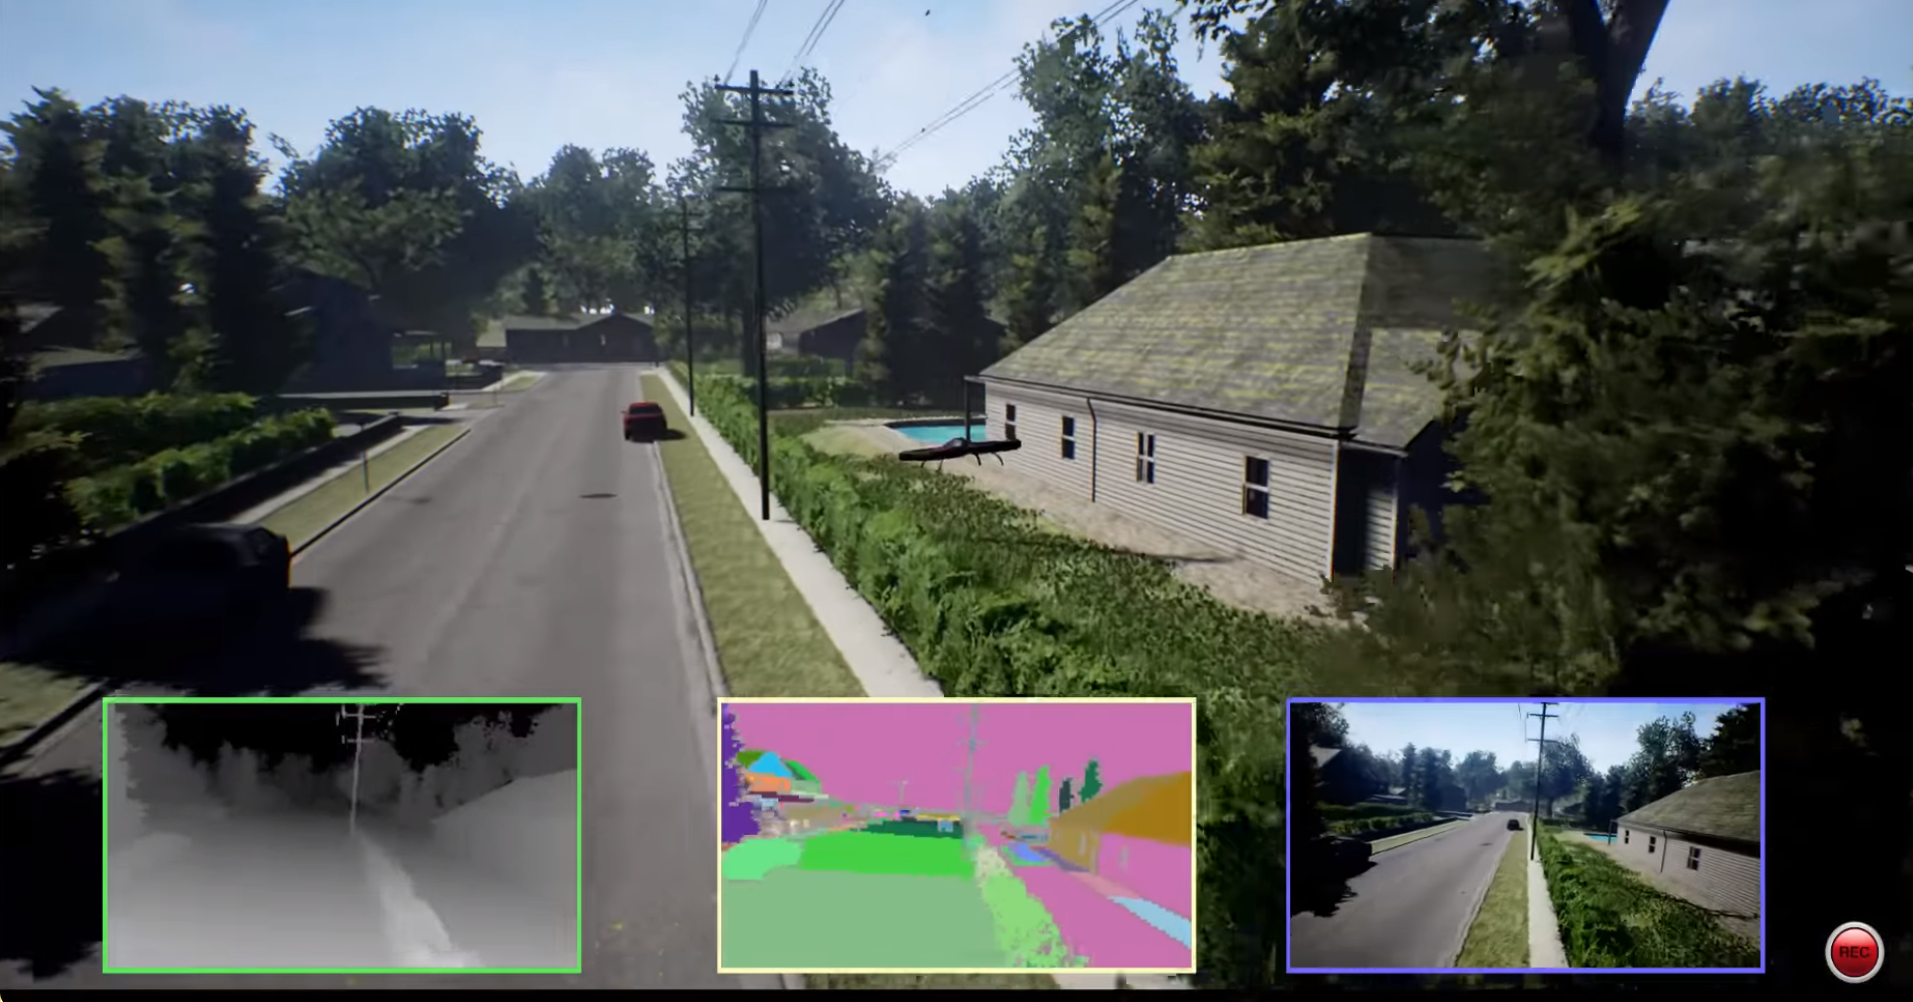
\includegraphics[width=0.8\textwidth]{airSim.png}
    \attribution{https://microsoft.github.io/AirSim}
\end{center}

Кстати, в робототехнической среде (в частности, при разработке беспилотных автомобилей) считается незазорным использовать для сбора наборов синтетических данных, скажем, GTA 5 --- игра обеспечивает достаточное для практических целей качество графики, разнообразные окружения и т.п., так что почему нет. 

В мире программных робототехнических платформ абсолютно доминирует ROS (Robot Operating System).
Несмотря на своё название, ROS --- это не операционная система, а промежуточное программное обеспечение (middleware), обеспечивающее запуск и распределённую работу робототехнических алгоритмов, плюс имеющее обширную библиотеку готовых алгоритмов, средства интеграции с аппаратными устройствами и даже симуляторами.
Прикладной программист под ROS пишет (или конфигурирует готовые) \emph{узлы}, что-то вроде микросервисов, реализующих какую-точ часть функциональности системы. 
Узлы могут общаться друг с другом с помощью \emph{топиков} --- типизированных каналов, на которые узлы могут подписываться и куда писать сообщения.
Напрямую узлы взаимодействовать не могут, только через топики (то есть ROS реализует классический событийный архитектурный стиль с шиной).
Собственно ROS делает так, чтобы общение узлов происходило прозрачно --- запущены узлы на одном устройстве или где-то далеко в сети (например, на компьютере, а не на роботе вовсе).
ROS 2 считается актуальной и более прогрессивной версией ROS, поскольку обеспечивает полную децентрализацию (все узлы равноправны) и работает под разными ОС (ROS 1 работал только под Linux), однако многие до сих пор используют ROS 1.

Вот схема архитектуры ROS:

\begin{center}
    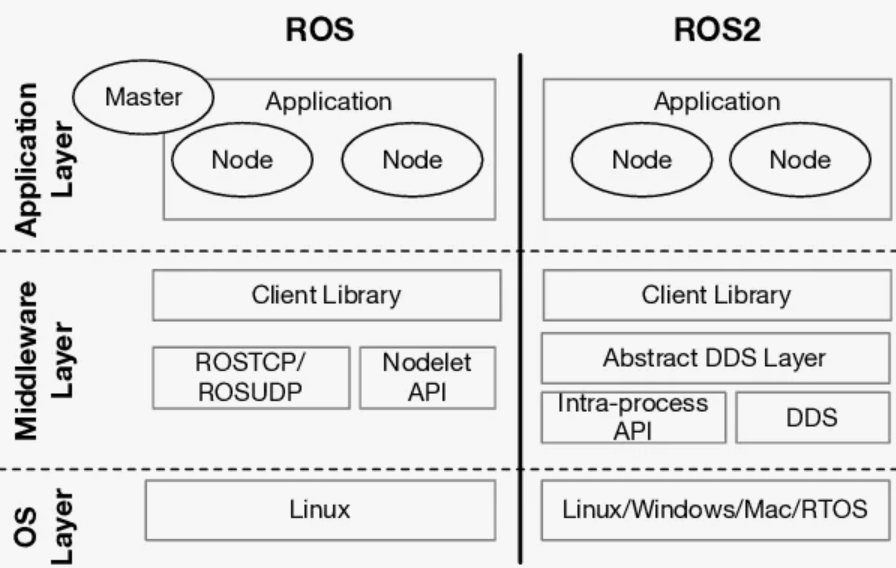
\includegraphics[width=0.7\textwidth]{ros.png}
    \attribution{\url{https://www.researchgate.net/figure/Comparison-between-ROS-and-ROS2_fig4_335382592}}
\end{center}

Вообще ROS предполагается использовать для прототипирования и научных исследований, но в продакшене он тоже в достаточных количествах присутствует --- например, внезапно, беспилотные карьерные самосвалы где-то на крайнем севере России работают именно на ROS.

Есть ещё некоторое количество относительно известных платформ, которые более низкоуровневые, чем ROS, и более легковесны, например:

\begin{itemize}
    \item Player --- часть технологического стека Player/Stage/Gazebo, умеет сопрягать реальные устройства с симулятором для, например, совместной работы реальных и симулируемых устройств;
    \item RT-middleware --- стандарт на распределённую робототехническую платформу от того самого OMG, что поддерживает UML;
    \item YARP --- библиотека для распределённых вычислений в робототехнике.
\end{itemize}

Тут они приводятся скорее для полноты картины, по умолчанию аппаратная платформа, если голая ОС или \enquote{железо} уже не устраивают --- ROS. Если ROS уже не подходит, к этому моменту вы уже знаете про другие проекты и можете сами сделать осознанный выбор.

\section*{Заключение}

Большая часть изложения выше и большая часть изображений взяты из книжки Roland Siegwart, Illah Reza Nourbakhsh, Introduction to Autonomous Mobile Robots, MIT Press, 2004, 321 pages (она вроде как переиздавалась, тут используется издание 2004 года, новое вполне может быть лучше). Книжка старая, написана до хайпа по ML, поэтому рассматривает только классические алгоритмы, но очень годная и как введение в робототехнику очень хороша. Может, в ней несколько больше математики, чем любят на программной инженерии, но всё же, очень рекомендую. Думаю, знания, содержащиеся там, вполне соответствуют уровню, которым прилично владеть в робототехнике любому грамотному программному инженеру с широким кругозором, или минимуму знаний для того, кто хочет заниматься исследованиями в робототехнике. Прочитаете книжку --- можно смело в магистратуре заниматься робототехникой.

Эта книга --- основная рекомендованная литература курса, большую часть докладов стоит делать именно по ней.

\end{document}
